
\chapter{Full Detector Simulation And Evaluation}\label{chp:DataAnalysisTechniques}

In this chapter the individual effects from each component are added to model the mass increase. This allows for a machine learning study to asses whether machine learning is a suitable technique for the trigger data for the upgraded (VIDARR) detector. The results from a current technique suggests that machine learning is effective at finding suitable boundaries and reducing the dimensionality of trigger data but that complex boundaries are unnecessary. Then cosmic muons are modelled using the CRY library \cite{ieee_cry_2007} and once they have been successfully modelled a cosmic muon tracker is built using a simulation of a hemispherical source of cosmic muons. This tracker does not seem to add any significant bias to the reconstruction of cosmic muon events.

\section{Modelling The Mass Increase}
The number of layers in the initial detector was 49 out of a possible 70. The upgrade will therefore add $\sim$ 43\,\% additional mass into the detector compared to the initial detector. In reality, out of a possible 1862 channels in the prototype, only 1793 were instrumented due to limitations in securing enough parts. Nevertheless, the simulation will focus on the theoretical maximum number of bars in both cases for the sake of simplicity. During the deployment at Wylfa there was a measurement of about 200 electron anti-neutrino candidates a day \cite{Carroll_2018} (figure \ref{fig:prototypeMeasumentFlux}), and so from the upgraded detector it is reasonable to assume a rate of $\sim$ 300 electron anti-neutrino candidates a day with the additional mass. In addition, the quality of each event will also improve as more of the energy from the 8\,MeV gamma-ray cascade is kept within the instrumented volume of the detector. The ratio of the energy deposited and the energy released in the detector will be considered the ``containment'' of the cascade where containment of 100\,\% would mean 100\,\% of the energy is deposited in the detector. And as figure \ref{fig:containment_comparison} shows the containment improves with more mass and has a lower surface-to-volume ratio. %In figure \ref{fig:containment_comparison} it can be seen that the quality of the containment increases when the additional mass has been added. 

\begin{figure}[!h]
 \centering
 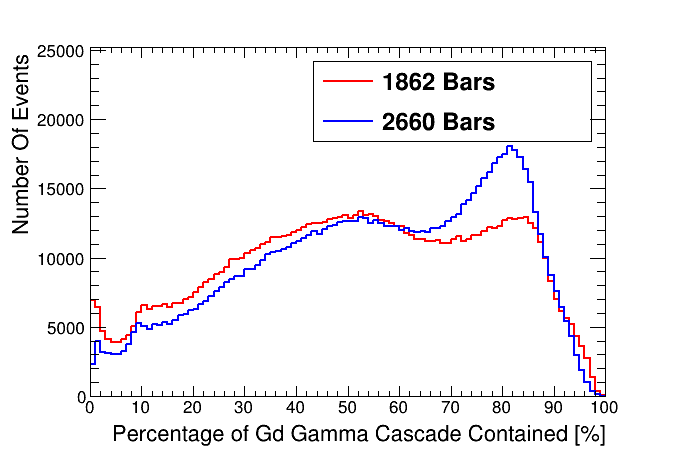
\includegraphics[width=0.7\linewidth]{Chapter4/Figs/cascadeContainmentCompare.png}
 \captionof{figure}[Gd gamma-ray containment for the original and upgraded detector.]{Gd gamma-ray containment for 1862 bars (49 layers) and 2660 bars (70 layers) expressed as a percentage. The quality of the events improves with the taller detector as expected. Cascade containment $\leq$ 0.1\,\% is treated as 0\,\%. }
 \label{fig:containment_comparison}
\end{figure} 

When simulating electrons and positrons with 0\,MeV -- 10\,MeV kinetic energy, the amount of energy contained inside is $\sim$ 100\,\% but slowly decreases as the energy increases. The amount of energy generated (E$_\textrm{{Gen}}$) versus the energy deposited  (E$_\textrm{{Dep}}$) for these two particles is shown in figure \ref{fig:recon_gen_ele_pos}. The loss of energy matches that seen in section \ref{sec:GEANT4Simulation_quenchingLoss}, where most of the energy lost is due to scattering and straggling, but quenching has minimal impact on the visible energy. Then positron particles are simulated from 1\,MeV -- 10\,MeV to determine detection efficiencies in figure \ref{fig:2000_3000_p_secs} for both 1862 bars (figure \ref{subFig:2000_p_sec}) and 2660 bars (figure \ref{subFig:3000_p_sec}) above a 0.1\,MeV threshold. In both cases the efficiency does not fall below 99\,\% for positrons. This is due to the fact that positrons typically do not escape the detector without depositing $>$ 0.1\,MeV in at least a single bar. As such positron efficiencies are mostly independent of the overall detector mass and size but are extremely high regardless of the mass increase.  

\begin{figure}[!h]
 \centering
 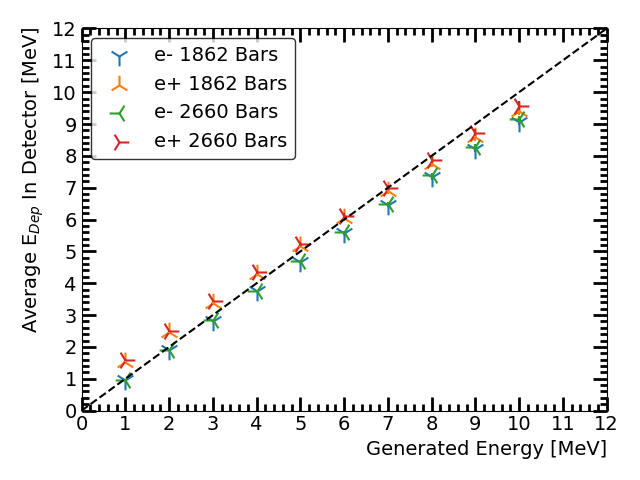
\includegraphics[width=0.7\linewidth]{Chapter4/Figs/summedVsTruth_1862_2660_e-e+_eBars_Adjusted.png}
 \captionof{figure}[Energy response for simulated electrons and positrons in the upgraded VIDARR detector.]{Energy response of the simulated detector for both electrons and positrons in the full detector in comparison to E$_\textrm{{Dep}}$ = E$_\textrm{{gen}}$. The positron's annihilation gamma-rays causes E$_\textrm{{Dep}}$ $>$ E$_\textrm{{Dep}}$ at low generated energies. Generated energy has no error. The number of generated events per point is 10$^5$. Errors for E$_\textrm{{Dep}}$ are determined by standard error on the mean and are small but are shown on this plot.}
 \label{fig:recon_gen_ele_pos}
\end{figure} 

\begin{figure}[!h]
\centering
\begin{subfigure}{.5\textwidth}
  \centering
  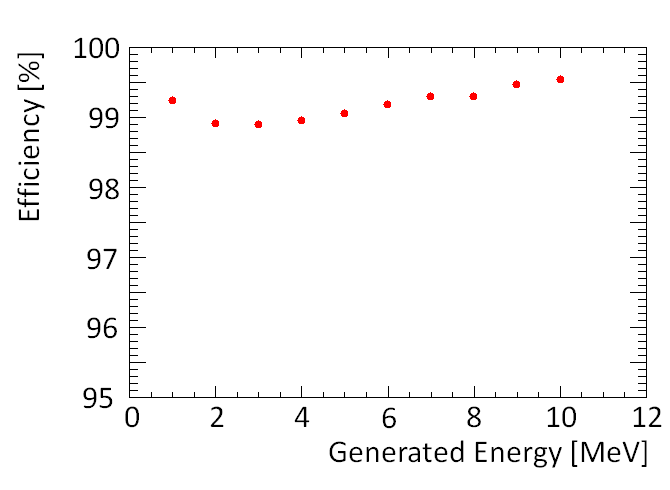
\includegraphics[width=\linewidth]{Chapter4/Figs/Raster/year1Plots/2000_1-10MeV_sec_p_spread_run_medText.png}
  \captionsetup{width=.9\linewidth}
  \caption{}
  \label{subFig:2000_p_sec}
\end{subfigure}%
\begin{subfigure}{.5\textwidth}
  \centering
  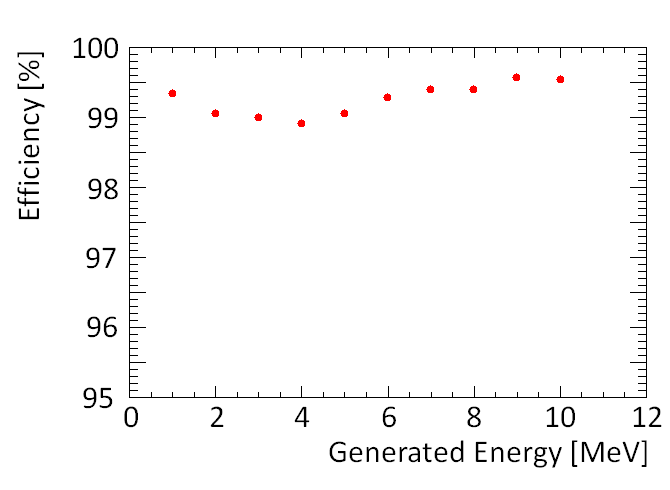
\includegraphics[width=\linewidth]{Chapter4/Figs/Raster/year1Plots/3000_1-10MeV_sec_p_spread_run_medText.png}
  \captionsetup{width=.9\linewidth}
  \caption{}
  \label{subFig:3000_p_sec}
\end{subfigure}
\caption[Positron hit efficiencies for the original and upgraded detector.]{The percentage of generated positrons that deposit > 0.1\,MeV in the detector. (a) shows the original 1862 barred detector (b) shows the upgraded 2660 barred detector. The hit efficiencies are almost identical for each, the mass increase has no impact on positron hit efficiencies. The efficiency errors are of the order $\sim$ $10^{-3}$\,\%.}%{Positron hit efficiencies for the original 1862 bar detector (a) and the upgraded 2660 bar detector (b) above a 0.1\,MeV threshold both have $\sim$ 99\,\% efficiencies are similar in both errors are too small to be shown. Generated energy errors are non existent and efficiency errors are of the order $\sim$ $10^{-3}$. }
\label{fig:2000_3000_p_secs}
\end{figure}

\clearpage
\section{Machine Learning Neutron Trigger}\label{sec:MachineLearningTrigger}
The exact trigger configuration for the upgraded detector is in a state of flux as it will be fully implemented as calibration data becomes available. However, for the following work it is assumed that two distinct thresholds will be used for reactor monitoring operations. In addition, the FPGA boards allow for determining the summed energy above each of these thresholds and the number of bars hit above each of these thresholds. The lower threshold chosen was 2.5\,PE (0.1\,MeV) as this is the lowest threshold willing to be entertained to mitigate dark noise. The upper threshold chosen was 12.5\,PE (0.5\,MeV) as going higher than this risks excluding too many hits from the Gd cascade. The four potential variables are shown in figure \ref{fig:preTriggerData}. Of the four variables shown in figure \ref{fig:preTriggerData} only the number of bars hit above 2.5\,PE (figure \ref{subFig:preTrigNba2.5}) clearly separates between neutrons and potential background. This particular problem is best solved by machine learning classification. This is where an algorithm is given a data set and corresponding set of keys as to which is signal and which is noise, then based on the previous data is able to predict whether a future data point is signal or noise.
\begin{figure}[!h]
\centering
\begin{subfigure}{.49\textwidth}
  \centering
  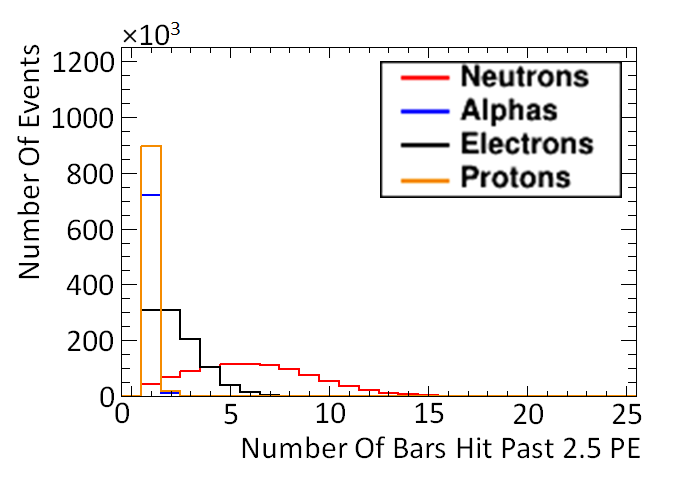
\includegraphics[width=\linewidth]{Chapter4.5/Figs/preTrigNba2.5.png}
  \captionsetup{width=.9\linewidth}
  \caption{}
  \label{subFig:preTrigNba2.5}
\end{subfigure}%
\begin{subfigure}{.49\textwidth}
  \centering
  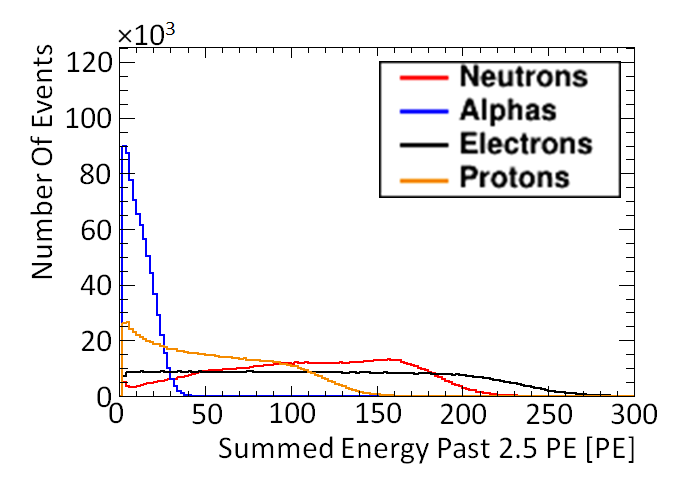
\includegraphics[width=\linewidth]{Chapter4.5/Figs/preTrigSea2.5.png}
  \captionsetup{width=.9\linewidth}
  \caption{}
  \label{subFig:preTrigSea2.5}
\end{subfigure}
\begin{subfigure}{.49\textwidth}
  \centering
  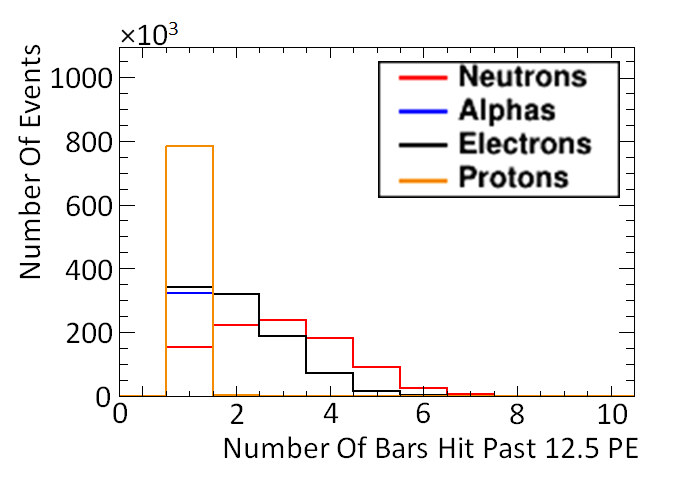
\includegraphics[width=\linewidth]{Chapter4.5/Figs/preTrigNba12.5.png}
  \captionsetup{width=.9\linewidth}
  \caption{}
  \label{subFig:preTrigNba12.5}
\end{subfigure}
\begin{subfigure}{.49\textwidth}
  \centering
  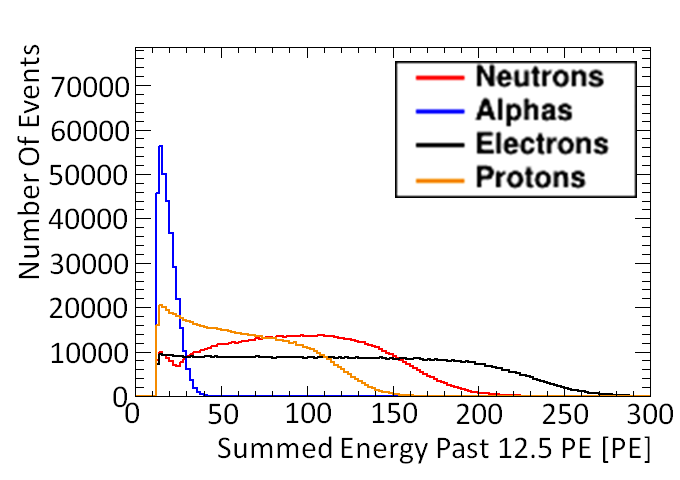
\includegraphics[width=\linewidth]{Chapter4.5/Figs/preTrigSea12.5.png}
  \captionsetup{width=.9\linewidth}
  \caption{}
  \label{subFig:preTrigSea12.5}
\end{subfigure}
\caption[Generated pre trigger data for neutrons, alphas, electrons and protons.]{Generated pre-trigger data for neutrons, alpha particles, electrons and protons. Two thresholds were chosen to help separate the data 2.5\,PE (0.1\,MeV) and 12.5\,PE (0.5\,MeV). The trigger should have access to the summed energy and number of bars above each of these thresholds. (a) number of bars hit above 2.5\,PE, (b) summed energy above 2.5\,PE, (c) number of bars hit above 12.5\,PE, (d) summed energy above 12.5\,PE.}
\label{fig:preTriggerData}
\end{figure}

%As a result a manual attempt using all hits above 4 bars or summed energies below the line $E^{12.5\,\textrm{PE}}_\textrm{Summed} \leq E^{2.5\,\textrm{PE}}_\textrm{Summed} - 12.5\,PE$ The selection went as required either >= 4 bars must be hit \textbf{or} $E^{12.5\,\textrm{PE}}_\textrm{Summed} \leq E^{2.5\,\textrm{PE}}_\textrm{Summed} - 12.5\,PE$. 
But first a manual attempt to separate the data using two selection criteria (``cuts'') was attempted as described by equation \ref{equ:manualCuts}. This was to gauge where the minimum expected performance of a machine learning classifier should be.  
\begin{equation}
    \textrm{Bars}^{2.5\,\textrm{PE}}_\textrm{Number Hit} \geq 4 ~~\textbf{or}~~ \textrm{Energy}^{12.5\,\textrm{PE}}_\textrm{Summed} \leq \textrm{Energy}^{2.5\,\textrm{PE}}_\textrm{Summed} - 12.5\,\textrm{PE}. 
    \label{equ:manualCuts}
\end{equation}
These cuts include the detector effects mentioned in chapter \ref{chp:GEANT4Simulation}. This selection resulted in an efficiency of 59.8\,\% and a purity of 95.5\,\%. These values were somewhat disappointing, a trigger should optimise for efficiency rather than purity. These manual cuts sacrifice efficiency for purity. But it is possible that optimising for the Gd cascade signal will result in higher purity than efficiency regardless of the selection criteria due to how the distributions overlap. As a result an investigation using every possible combination was required. These different combinations are represented by a notation following the pattern $n$C$r$: 4C1 (4 choices), 4C2 (6 choices), 4C3 (4 choices), and 4C4 (1 choice). Determining which dimension, with each dimension representing one variable, combination is relevant is important as reducing dimensional complexity is highly desirable. A primary motivation is avoiding the ``curse of dimensionality'' \cite{taylor2019applications_cofD} where data is separable because it becomes more sparsely separated as the number of dimensions increases. Also, the fewer dimensions, the easier the real-world implementation of the trigger will be, which is important to reduce sources of potential errors and minimise computational requirements. For example, the manual cuts use three dimensions, two of which are the summed energy which introduces potential issues as calibrating $\sim$ 15 hits (see figure \ref{subFig:preTrigNba2.5}) and summing them has a much greater chance to introduce errors than looking for a number of hits above a given threshold. Therefore, an algorithm that could reliably find good separation between data sets with the minimal number of dimensions was sought after. This goal would be well met via machine learning. But great care had to be taken such that the chosen algorithm was not too simple i.e. unable to find good separation or too complex i.e requiring excessive development time. 
\\\\There are several machine learning techniques available to analyse different types of data. Typically the physics field uses decision trees (DT), k-nearest neighbours (KNN), and deep learning neural networks (DLNN). One technique which is often neglected is the support vector machine (SVM) \cite{Boser92atraining}, \cite{cortes1995support}. An SVM is a linear classifier that uses particular points (support vectors) in two data sets to find the best separating ``hyperplane'' an n-dimensional line that finds the maximum separation between the two data sets (see figure \ref{fig:svmBoser92LinearSVM}). The margins separating the data sets (M$^*$ in figure \ref{fig:svmBoser92LinearSVM}) are only determined by the support vectors, other points that are not support vectors are ignored when creating the boundary. Whilst the SVM is a linear classifier it is possible to use a function to distort non-linear data such that it becomes linearly separable. These functions are called kernels and an example of how they are used can be seen in figure \ref{fig:kernelRBF_fromWeB}. The kernel used in figure \ref{fig:kernelRBF_fromWeB} is the radial base function (RBF) kernel described by equation \ref{equ:RbfKernelFunc}. The method of transforming data through a kernel via the ``kernel trick'' is well established and has been a common technique since at least 1992 \cite{Boser92atraining}.
% Using simulated data it is possible to test whether a machine learning trigger would be advantageous to the analysis. The machine learning technique considered the most appropriate was the Support Vector Machine (SVM) \cite{Boser92atraining} \cite{cortes1995support}, as SVMs were compared to several other simple techniques typically used in physics namely a decision tree and k-nearest neighbours (see figure \ref{fig:sklearnReleventExamples}). As seen in figure \ref{fig:sklearnReleventExamples} the SVM linearly or with a kernel. The radial basis function (RBF) kernel is one of the most common. In figure \ref{fig:sklearnReleventExamples} the generalised boundaries, high accuracy, and well-defined projection space seen in the RBF SVM make it the clear standout. The SVM utilises the RBF kernel via the kernel trick since at least 1992 \cite{Boser92atraining}. 
% \\\\SVMs work by finding the best separating hyperplane between two opposing data sets. In figure \ref{fig:svmBoser92LinearSVM} the best separating hyperplane is calculated for a simple data set. The SVM works by finding the maximum distance between each data set and creating an n-dimensional line the ``hyperplane'' to separate the data. In order to separate non-linear data the kernel trick is used which figure \ref{fig:kernelRBF_fromWeB} shows. Figure \ref{fig:kernelRBF_fromWeB} also shows how two different kernels achieve the same result. How the decision surface is manipulated to separate data sets is shown in figure \ref{fig:kernelRBF_fromWeB}. As figure \ref{fig:kernelRBF_fromWeB} shows the kernel transforms the data set so it becomes linearly separable for the SVM. A further test of the SVMS's capabilities is done in figure \ref{fig:svmExp_GausseExamples} which tests the separation of multiple Gaussian data sets from 2D exponential noise. This is as complex ass trigger data could reasonably be expected to be. This means that the SVM should be suitable for separating neutron trigger data. 
% \\\\An SVM is also convexly optimised which means the solutions are easier to solve as there is only one global minimum \cite{cortes1995support}. This feature allows SVMs to train on sparse data sets with low statistics. SVMs are fast to train on small data sets but as data sets grow larger the squared nature of the SVM solution increases training times dramatically \cite{cortes1995support}. This means that for data with many dimensions and many statistics training times and memory usage can be very high to the point of being unusable \cite{cortes1995support}. Data must also be completely labelled and optimisation for training whilst possible through sequential minimal optimisation is somewhat limited \cite{platt1998sequential}. These drawbacks are not a significant issue for the trigger data but they should be bared in mind for more complex cases such as image recognition.
\begin{equation}
K(\mathbf{x,x'}) = \exp{(\gamma \mathbf{x \cdot x'})} - 1
\label{equ:RbfKernelFunc}
\end{equation}

\begin{figure}[!h]
\centering
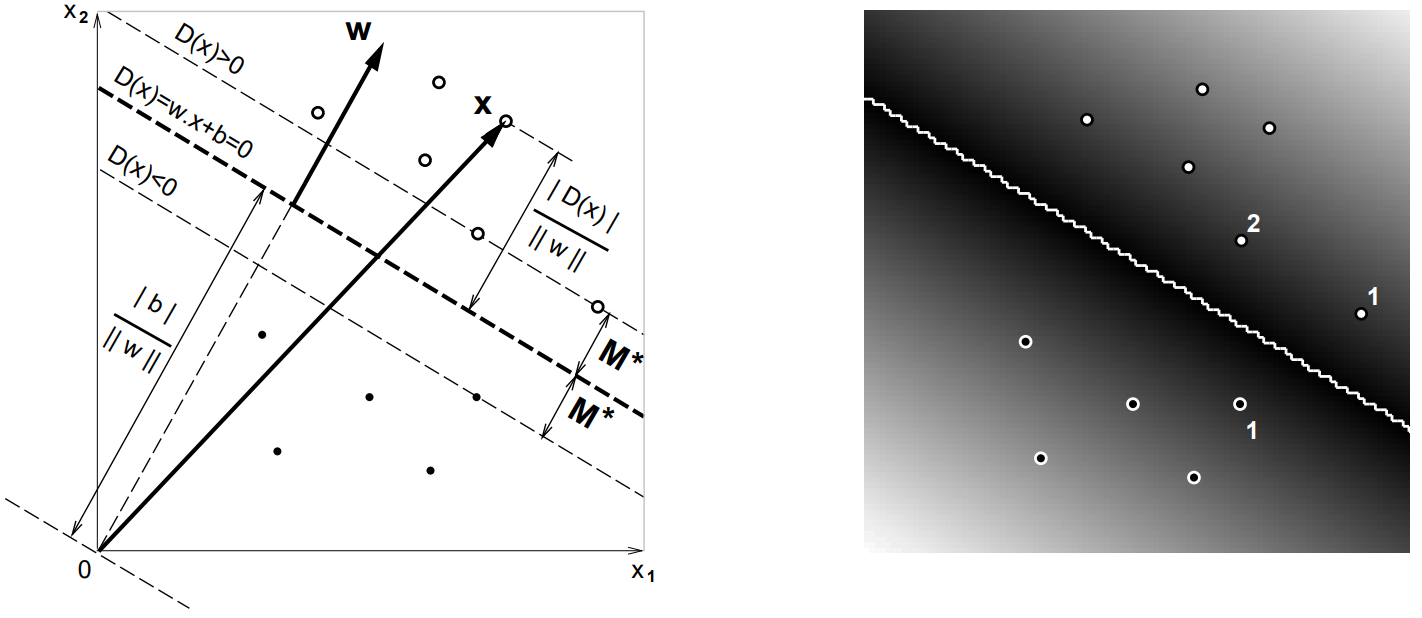
\includegraphics[width=0.9\linewidth]{Chapter4/Figs/Raster/svmLinAndRbf/svmBoser92LinearSVM.png}
\captionof{figure}[An example of how a support vector machine separates linear data.]{An example of how a support vector machine (SVM) separates two different distributions that are linearly separable. The maths behind the classifier finds the best separating line/hyper-plane between two distributions. From \cite{Boser92atraining}.} 
\label{fig:svmBoser92LinearSVM}
\end{figure}

% \begin{figure}[!h]
% \centering
% 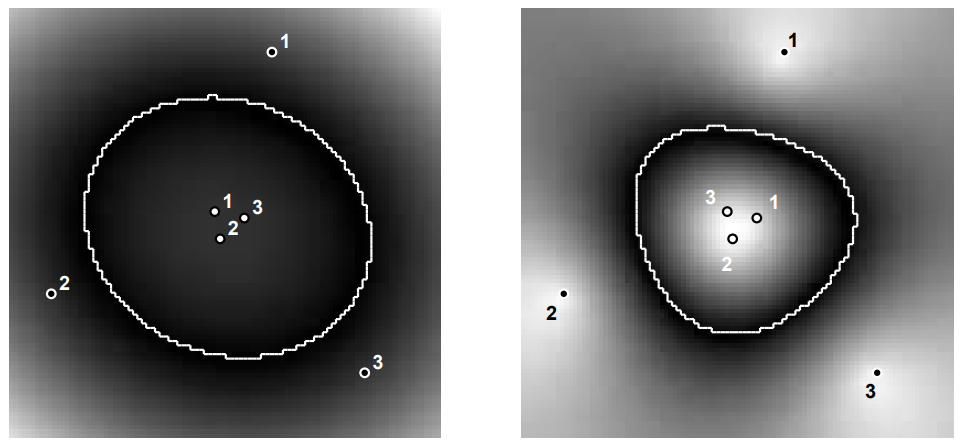
\includegraphics[width=0.7\linewidth]{Chapter4/Figs/Raster/svmLinAndRbf/svmBoser92KernelSVM.png}
% \captionof{figure}{How a support vector machine (SVM) operates with a kernel being applied using a squared polynomial kernel on the left and a radial basis function (RBF) on the right. By using the ``kernel trick'' it is possible to separate non-linear data. From \cite{Boser92atraining}.} 
% \label{fig:svmBoser92KernelSVM}
% \end{figure}

\begin{figure}[!h]
\centering
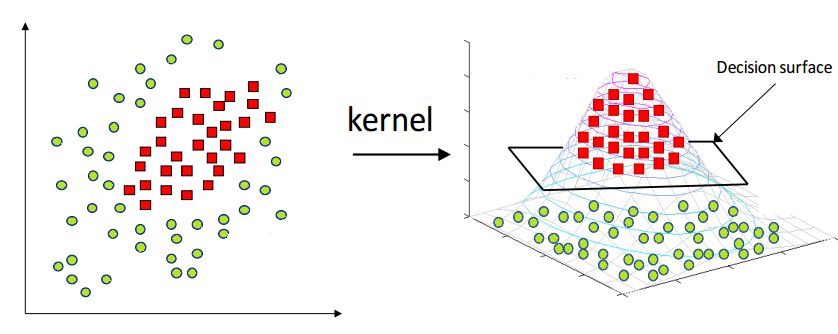
\includegraphics[width=0.9\linewidth]{Chapter4/Figs/Raster/svmLinAndRbf/kernelRBF_fromWeB.png}
\captionof{figure}[An online kernel trick example.]{An online example that shows how the kernel trick is used to make non-linear data linearly separable by transforming it through a kernel. From \cite{kernelTrickWeb}.} 
\label{fig:kernelRBF_fromWeB}
\end{figure}
 
A direct comparison between DT, KNN, linear (no kernel) SVM and RBF SVM classifiers is done in figure \ref{fig:sklearnReleventExamples}. In figure \ref{fig:sklearnReleventExamples}, the generalised boundaries, high accuracy and well defined projection space of the RBF SVM make it the clear standout for our application. However, each machine learning technique has its drawbacks. Whilst SVMs are convexly optimised, only having one global minimum \cite{Boser92atraining} this comes at the cost of parallelisation. In order to achieve the well-defined projection space with such a simple algorithm, the SVM must be able to observe the whole of the data at once. This is somewhat mitigated by sequential minimal optimisation \cite{platt1998sequential} but not completely. This means that for very large data sets with thousands of dimensions an SVM might not always be suitable as training times become too long. However, the trigger data for the VIDARR detector only has a maximum of four dimensions shown in table \ref{tab:triggerDims}. Data must also be labelled for SVMs as well but this is not a significant limitation for VIDARR data sets, as labelling of data is likely to be done regardless of machine learning.
 
\begin{figure}[!h]
\centering
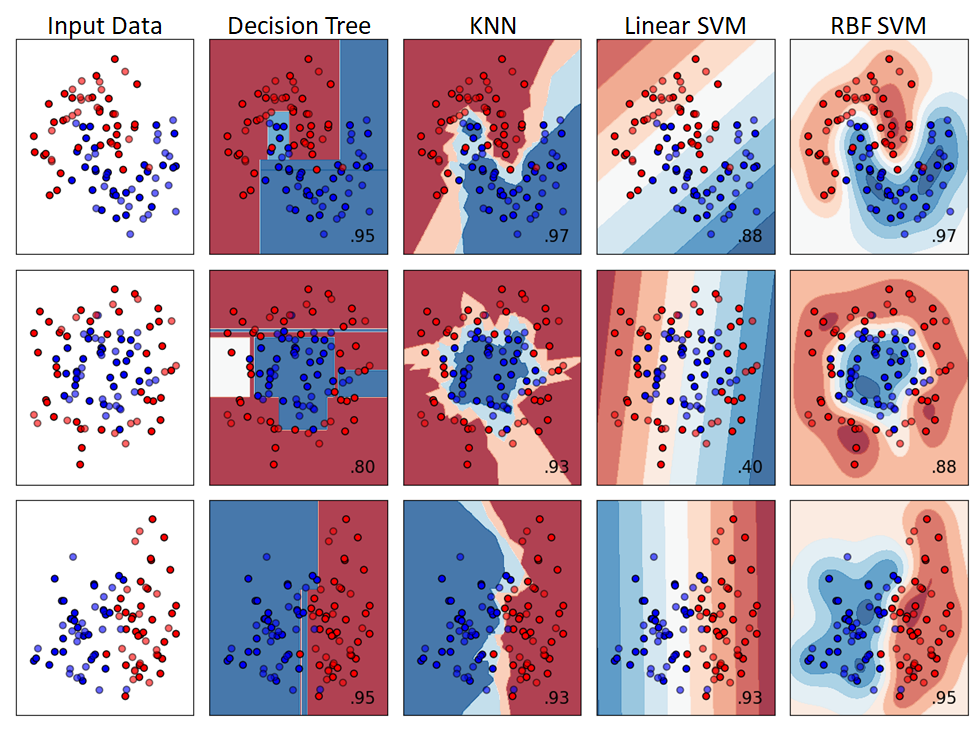
\includegraphics[width=0.9\linewidth]{Chapter4/Figs/Raster/svmLinAndRbf/sklearnReleventExamplesMedText.png}
\captionof{figure}[Example classifiers taken from \texttt{scikit-learn} that show different techniques.]{Some example classifiers taken from \texttt{scikit-learn} that show how different techniques draw boundaries and their projection spaces. Decision trees and k nearest neighbours are common simplistic classifiers used in physics but the boundaries they produce are often susceptible to over-training. The linear SVM is generalised but is quite limited in its utility. The SVM with the RBF kernel consistently draws the most accurate boundaries and they are well generalised. The accuracy of each technique is shown in the bottom right of each plot. From \cite{scikit-learn}.} 
\label{fig:sklearnReleventExamples}
\end{figure}

\begin{table*}[!h]
\centering
\begin{tabular}{lcc}  
\toprule
Dimension               & Th 2.5\,PE (0.1\,MeV) & Th 12.5\,PE (0.5\,MeV)\\
\midrule
\# of Bars Hit Above Th &  NBATh$_{2.5}$        & NBATh$_{12.5}$\\
Summed Energy Above Th  &  SEATh$_{2.5}$        & SEATh$_{12.5}$\\
\bottomrule  
\end{tabular}
\caption{A table showing the 4 dimensions that the trigger can have. The word threshold is abbreviated to Th for convenience.}
\label{tab:triggerDims}
\end{table*}

%Nyström
% Figures \ref{fig:sklearnReleventExamples} \ref{fig:svmBoser92LinearSVM} \ref{fig:kernelRBF_fromWeB} \ref{fig:kernelRBF_fromWeB} \ref{fig:svmExp_GausseExamples} are sufficient reason to believe that an SVM with an RBF kernel should be a suitable classifier for separating trigger data that only has four dimensions. The four dimensions that need to be optimised are: the summed energy above a threshold of 2.5\,PE (0.1\,MeV), summed energy above a threshold of 12.5\,PE (0.5\,MeV), Numbers of bars hit above a threshold of 2.5\,PE (0.1\,MeV), Numbers of bars hit above threshold 12.5\,PE (0.5\,MeV). The libraries used were LIBSVM and LIBLINEAR both of which are highly provident and often cited as the reason for the SVMs gain in popularity \cite{chang2011libsvm} \cite{fan2008liblinear} \cite{murty2016support}. The wrapper in sci-kit learn was the preferred method due to its ease of use and its convenient application of the Nystrom approximation \cite{williams2001using} of the kernel. The Nystroem approximation is useful as the amount of computation required for a complete kernel SVMs scales $\sim$ O (n$^3$) where n is the number of training examples \cite{williams2001using}. By using a sample of size m to compute an approximation of the kernel the amount of computation required scales $\sim$ O (m$^2$n) instead \cite{williams2001using}. This approach will work even when m $\ll$ n \cite{williams2001using}. The example data shown in figure \ref{fig:svmExp_GausseExamples} shows how LIBLINEAR when combined with with an RBF Nystroem approximated kernel performs in comparison to LIBSVM with a complete RBF kernel the boundaries are very similar. From this point, the LIBLINEAR library and the Nystroem approximation will be used to speed up training and to prevent memory overflow which can happen when the SVM isn't converging and when large data sets are used. The simulated data set has 1 million neutron signal events and 4 million background events.

There is also another issue when using a kernel SVM, the kernel itself greatly increases the computational requirement. A linear (no kernel) SVM requires computational power that scales $\mathcal{O}n^2$ (where $n$ is the number of training samples) \cite{cortes1995support}. But when a kernel is used the computational power required scales as $\mathcal{O}n^3$ instead \cite{williams2001using}. In order to mitigate this an approximate kernel is created via the Nyström method. By using a sample size of $m$ to compute this approximate kernel the computation requirement scales as $\mathcal{O}m^2n$ \cite{williams2001using}. This approach will work effectively even when $m << n$ \cite{williams2001using}. 
\\\\The kernel transformation is more complex than naively expected. In figure \ref{fig:svmExp_GausseExamples}, a simple transformation through a single point as demonstrated in figure \ref{fig:kernelRBF_fromWeB} would not give a clear separation. The RBF kernel (equation \ref{equ:RbfKernelFunc}) when projected back into 2D will only produce a circle when projected through a single point. In reality, the kernel is applied around every single point in the training data set. The SVM views all of these slices at once to create the boundary. It can be thought of as the SVM weighting each projected circle and choosing which pieces of each circle to keep and which to discard, thus allowing for the creation of almost any complex boundary. This is computationally expensive as this is transforming every single data point through a function. This is mitigated via the Gram matrix to some extent which allows for more efficient kernel computation \cite{williams2001using}. But this is $n^3$ complexity hence the use of the Nyström approximation of the Gram matrix to reduce computational load \cite{williams2001using}. 
\\\\Due to its preexisting implementation of the Nyström kernel approximation the wrapper \texttt{scikit-learn} was chosen as it saved development time \cite{scikit-learn}. \texttt{scikit-learn} uses LIBSVM \cite{chang2011libsvm} and LIBLINEAR \cite{fan2008liblinear} both of which are highly prominent and often cited as the reason for the SVM's gain in popularity \cite{murty2016support}. In figure \ref{fig:svmExp_GausseExamples}, a non-linear data set with two Gaussian signal distributions and an exponential distribution in (x,y) for noise is separated with LIBSVM using an RBF kernel (figure \ref{subFig:svmExp_2GausseExample}) and LIBLINEAR using an approximated Nyström kernel (figure \ref{subFig:exp_2NysGaussExample}). The example data in figure \ref{fig:svmExp_GausseExamples} shows how LIBLINEAR when combined with a Nyström approximated kernel performs to a similar standard to LIBSVM with a full RBF kernel, the resulting boundaries are extremely similar. It also shows that \texttt{scikit-learn}'s implementation of the Nyström method is accurate and reliable. From this point the LIBLINEAR library and the Nyström approximated RBF kernel will be used to speed up training and prevent an excess use of computational resource. Considering the strengths of SVMs, the low dimensionality of the trigger data, and the effective use of available computational resource, the approximate RBF SVM should is sufficient for separating out the 1 million generated signal events and the 4 million generated background events. 

\begin{figure}[!h]
\centering
\begin{subfigure}{.5\textwidth}
  \centering
  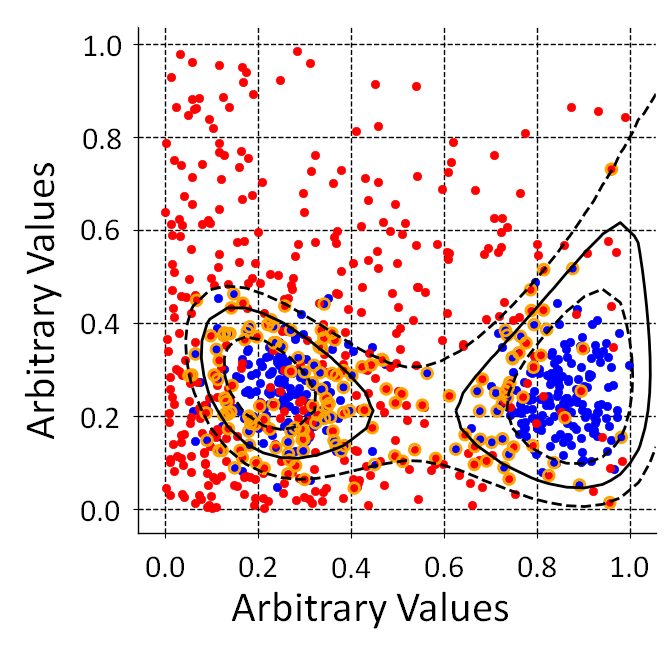
\includegraphics[width=\linewidth]{Chapter4/Figs/adjustedSvmPlots/adjusted_exp_2GaussExample.png}
  \captionsetup{width=.9\linewidth}
  \caption{}
  \label{subFig:svmExp_2GausseExample}
\end{subfigure}%
\begin{subfigure}{.5\textwidth}
  \centering
  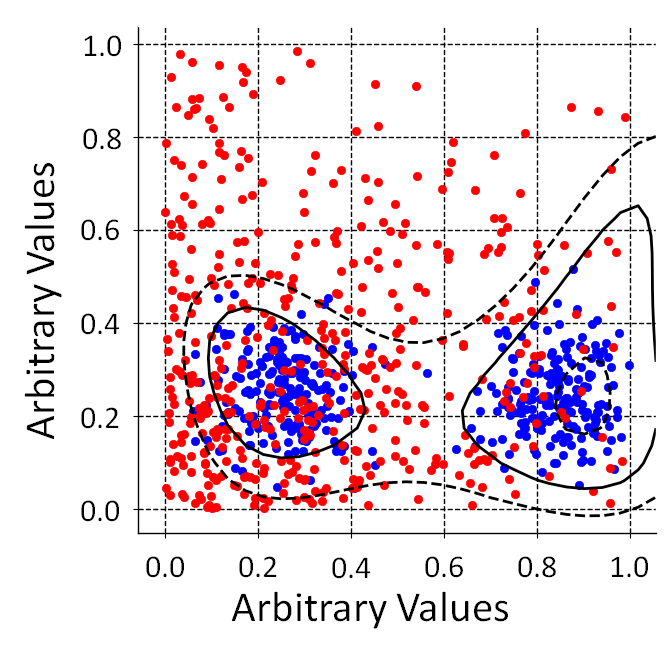
\includegraphics[width=\linewidth]{Chapter4/Figs/adjustedSvmPlots/adjusted_exp_2NysGaussExample.png}
  \captionsetup{width=.9\linewidth}
  \caption{}
  \label{subFig:exp_2NysGaussExample}
\end{subfigure}
\caption[SVM example separating two Gaussian data sets from exponential noise.]{SVM examples showing how to separate data sets with two Gaussian signals (blue) from exponential noise (red). For both an RBF kernel was used with c = 10$^3$ and $\gamma$ = 1. In (a) LIBSVM is used with an RBF kernel and support vectors are highlighted in orange. In (b) LIBLINEAR is used with a Nyström approximation of the RBF kernel with a sampling (m) of 100.}
\label{fig:svmExp_GausseExamples}
\end{figure}

RBF kernel SVMs have two factors that can be tuned to give more accurate results. The soft margin C and $\gamma$ which is part of the RBF kernel described by equation \ref{equ:RbfKernelFunc} \cite{Boser92atraining}. The soft margin C allows for the separation of data sets where there is overlap between the two data sets \cite{cortes1995support}. For the SVM this typically leads to larger margins considering more points in the construction of the hyperplane. $\gamma$ is the gradient of the deformation in the kernel and a higher value of $\gamma$ corresponds to higher non-linearity. Typically, C can vary from 10$^{-6}$ to 10$^6$ but can be even higher or even lower providing it is above 0. Values for $\gamma$ must also be above 0 and will vary depending on the linearity of the data. Figure \ref{fig:GammaCGridSearchExp2Gauss} shows the produced ranges of C and $\gamma$ for the non-linear data with significant overlap shown in figure \ref{subFig:exp_2NysGaussExample}. With this information, it can be seen that there is some overlap between the data sets  in figure \ref{subFig:exp_2NysGaussExample} and it is very non-linear so this search for relevant C and $\gamma$ values corroborates what can be intuitively discerned by looking at the example data in figure \ref{subFig:exp_2NysGaussExample}. In contrast, the generated neutron and noise data shows strong linearity as a low $\gamma$ value of 1 is preferred and has a small overlap as a high C value of 10$^6$ is preferred (see figure \ref{fig:GammaCGridSearchNeutron}). This shows that the generated neutron data is easy to separate with a linear classifier and using anything more complex than an SVM is unlikely to yield better results. This does not necessarily mean the data is 100\,\% linearly separable, but it does indicate the boundary formed is heavily dominated by a linear function. For example, this would be true of a boundary that curves towards the edges data sets at the edges but is otherwise linear. 

\begin{figure}[!h]
\centering
\begin{minipage}{.45\textwidth}
  \centering
  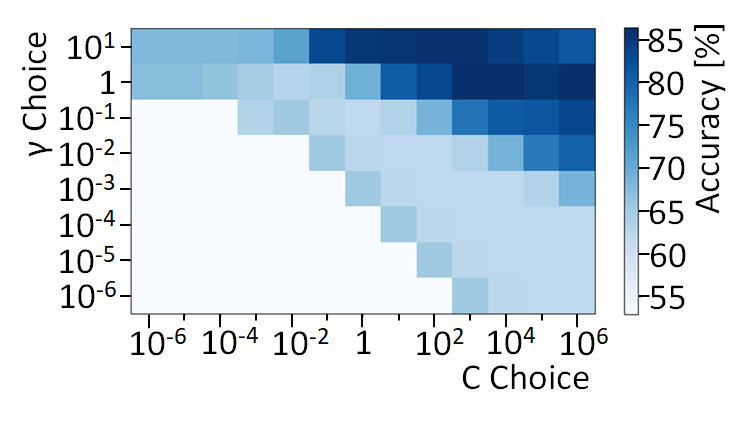
\includegraphics[width=\linewidth]{Chapter4/Figs/Raster/GammaCGridSearchExp2Gauss_adjustMedText.png}
  \captionof{figure}[SVM C and $\gamma$ grid search for exponential and Gaussian data.]{SVMs being trained on varying values of C and $\gamma$ for figure \ref{subFig:exp_2NysGaussExample}. Higher values of $\gamma$ represent non-linear data separation which the SVMs settle on. Higher values of C represent more overlap in the data. C choice is less clear but ultimately a higher value of C was settled due to a high preference for isolating boundaries as much as possible. A $\gamma$ = 1 and C = 10$^3$ was chosen.} 
  \label{fig:GammaCGridSearchExp2Gauss}
\end{minipage}%
\qquad
\begin{minipage}{.45\textwidth}
  \centering
  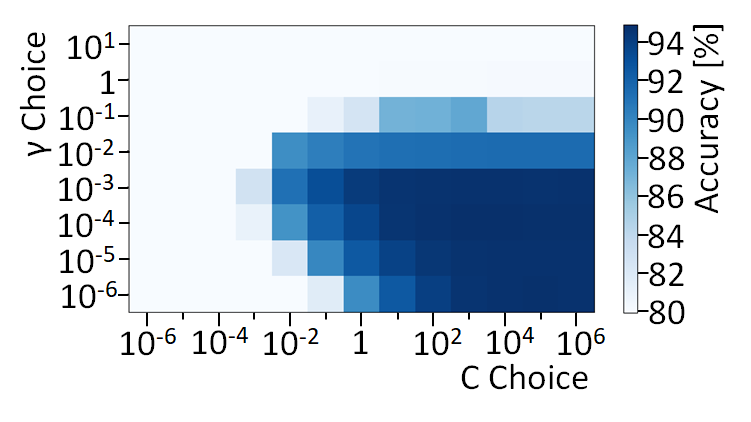
\includegraphics[width=\linewidth]{Chapter4/Figs/Raster/GammaCGridSearchNeutron_adjustMedText.png}
  \captionof{figure}[SVM C and $\gamma$ grid search for trigger data.]{SVMs being trained on varying values of C and $\gamma$ for figure generated background and neutron data. Lower values of $\gamma$ represent a linear data separation which the SVMs settle on. Higher values of C represent more overlap in the data. This data set is mostly linearly separable with minimal overlap. A $\gamma$ = 10$^{-6}$ and C = 10$^6$ was chosen.}
  \vspace{0.478cm} %1 line = 0.478cm % 2 lines = 0.956cm % 3 lines= 1.434cm % 4 lines = 1.912cm % 5 lines = 2.39cm
  \label{fig:GammaCGridSearchNeutron}
\end{minipage}
\end{figure}

%NBATh$_{2.5}$ & NBATh$_{12.5}$ SEATh$_{2.5}$ & SEATh$_{12.5}$\\
Once C and $\gamma$ have been chosen, a basic form of dimensional reduction was done to assess the impact of each dimension on the classifier (see figure \ref{fig:accNeutronSVMC1e6_g1e-6}). In figure \ref{fig:accNeutronSVMC1e6_g1e-6}, the addition of more dimensions beyond two does not increase accuracy suggesting that not all of the information provided by the emulated trigger is useful. This is also true for the efficiency as seen in figure \ref{fig:effNeutronSVMC1e6_g1e-6} and the purity as seen in figure \ref{fig:purNeutronSVMC1e6_g1e-6}. This shows that not only is the data largely linearly separable, it is actually 2D linearly separable, meaning it is extremely easy for any machine learning algorithm to separate. The powerful RBF SVM technique is already more than sufficient for this particular data set, hence why a DLNN has not been pursued. Following the notation using in table \ref{tab:triggerDims} The most accurate would choice of variables be the SEATh$_{2.5}$ + NBATh$_{2.5}$. However, the option NBATh$_{2.5}$ + NBATh$_{12.5}$ is easier to implement for the electronics on VIDARR. The drop in accuracy, efficiency, and purity is relatively low for this combination and therefore it is the preferred option. 

\begin{figure}[!h]
\centering
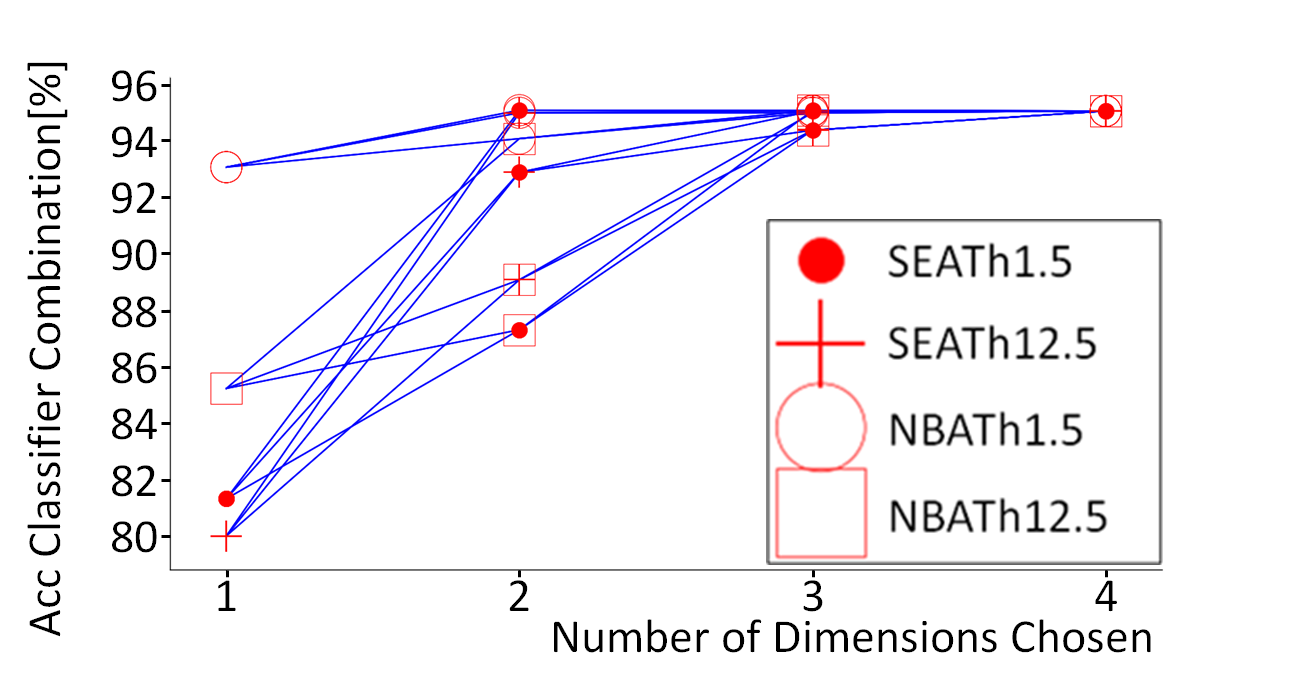
\includegraphics[width=0.8\linewidth]{Chapter4/Figs/Raster/accNeutronSVMC1e6_g1e-6MedText.png}
\captionof{figure}[Accuracy for different variables choices for SVM classifiers.]{Accuracy for Nyström SVM classifiers with approximate RBF kernels using a sampling of 100 for generated neutron and noise data. With C = 10$^6$ and $\gamma$ = 10$^{-6}$. Separation doesn't improve above 2 dimensions.} 
\label{fig:accNeutronSVMC1e6_g1e-6}
\end{figure}

\begin{figure}[!h]
\centering
\begin{minipage}{.45\textwidth}
  \centering
  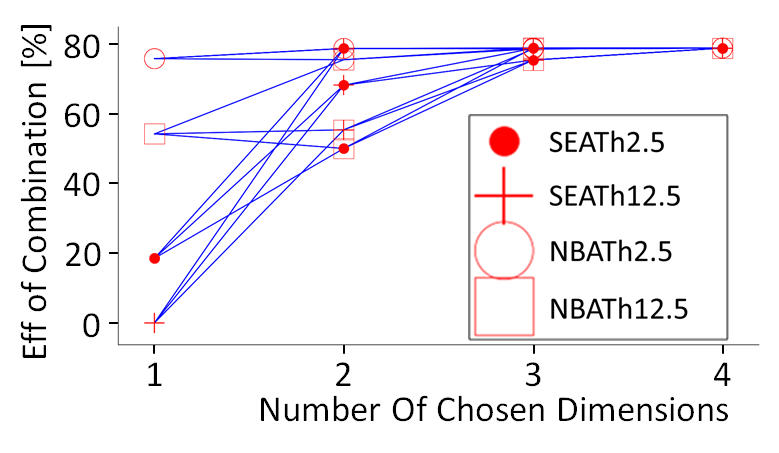
\includegraphics[width=\linewidth]{Chapter4/Figs/Raster/effCombSVMAdjustMedText.png}
  \captionof{figure}[Efficiency for different variables choices for SVM classifiers.]{Efficiency for Nyström SVM classifiers with approximate RBF kernels using a sampling of 100 for generated neutron and noise data. With C = 10$^6$ and $\gamma$ = 10$^{-6}$. Separation doesn't improve above 2 dimensions.} 
  \label{fig:effNeutronSVMC1e6_g1e-6}
\end{minipage}%
\qquad
\begin{minipage}{.45\textwidth}
  \centering
  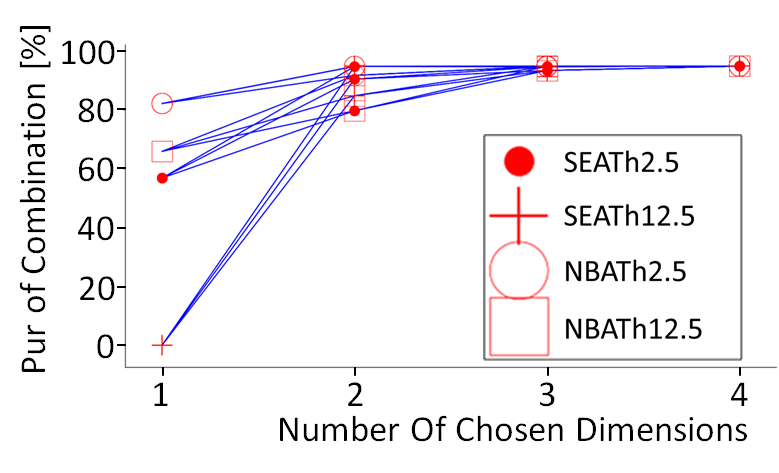
\includegraphics[width=\linewidth]{Chapter4/Figs/Raster/purCombSVMAdjustMedText.png}
  \captionof{figure}[Purity for different variables choices for SVM classifiers.]{Purity for Nyström SVM classifiers with approximate RBF kernels using a sampling of 100 for generated neutron and noise data. With C = 10$^6$ and $\gamma$ = 10$^{-6}$. Separation doesn't improve above 2 dimensions.}
  \label{fig:purNeutronSVMC1e6_g1e-6}
\end{minipage}
\end{figure}

The chosen classifier is seen in figure \ref{fig:signalAndNoiseNeutronSVM_C1e6_g1e-6}, which as figure \ref{fig:GammaCGridSearchNeutron} indicates is a linear classifier with minimal overlap between the signal and noise. In figure \ref{fig:signalAndNoiseNeutronSVM_C1e6_g1e-6} anything to the left of the line is considered a noise event and anything to the right of the line is considered a neutron event. The effect of these selection criteria can be seen in figure \ref{fig:summedEnergyPastTriggerGdDicebox} which shows the summed energy that passing the emulated trigger. The amount of summed energy passing the emulated trigger is overwhelmingly dominated by the 8\,MeV gamma-ray cascade from the neutron absorption. The only background events passing the emulated trigger are the electrons with high generated kinetic energies (above 4\,MeV) as seen in figure \ref{fig:GeneratedEnergyPastTriggerGdDicebox} but they are unlikely to be present when in sufficient quantities when the detector is deployed. 
\\\\These results show two points. The first is that the RBF SVM is significantly more capable than required for separating the trigger data. Thus indicating that other less advanced classifiers may also be suitable for separating the trigger data (such as the non-kernel SVM, KNN, and DT). The second is that the VIDARR trigger should be very effective at distinguishing the gamma-ray cascade from background expected at reactor sites. This is highly encouraging as it indicates that VIDARR's segmentation and technology are well suited to resolving the trigger signal from noise. It is possible that smaller segmentation would yield better results but considering the high simulated efficiency (75.3\,\%) it is unlikely to improve significantly. As a result, it can be concluded that VIDARR's segmentation and sensors are in a ``sweet spot'' where the signal is easy to separate whilst retaining relevant information. This conclusion will also be reinforced by the cosmic muon tomography results in chapter \ref{chp:cosmicMuonTomography}. A comparison of the manual selection and the SVM selection can be seen in table \ref{tab:svmSelection}, where the improvements the SVM makes to the efficiency are large ($> 15\,\%$) and the hit to purity is low ($< 4\,\%$) whilst using one fewer dimension. This justifies the use of the SVM machine learning technique as it has highlighted the optimal separation very efficiently. It is also possible to retrain the SVM within a short period of time ($<$ 3 hours) when the upgrade to the detector is finished and calibration data is taken.  

\begin{figure}[!h]
\centering
\begin{subfigure}{.5\textwidth}
  \centering
  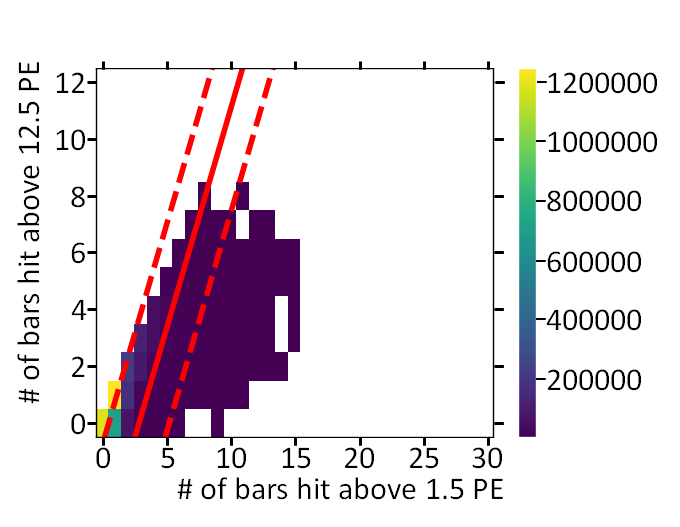
\includegraphics[width=\linewidth]{Chapter4/Figs/Raster/noiseNeutronSVM_C1e6_g1e-6MedText.png}
  \captionsetup{width=.9\linewidth}
  \caption{}
  \label{subFig:noiseNeutronSVM_C1e6_g1e-6}
\end{subfigure}%
\begin{subfigure}{.5\textwidth}
  \centering
  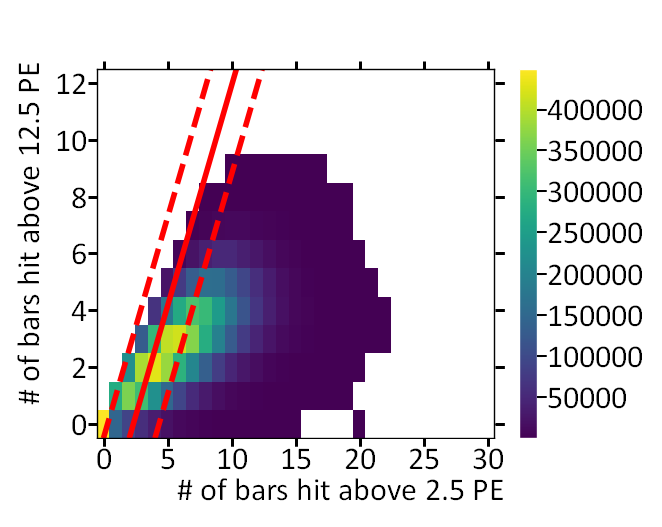
\includegraphics[width=\linewidth]{Chapter4/Figs/Raster/signalNeutronSVM_C1e6_g1e-6MedText.png}
  \captionsetup{width=.9\linewidth}
  \caption{}
  \label{subFig:signalNeutronSVM_C1e6_g1e-6}
\end{subfigure}
\caption[A 2D SVM classifier trained on generated neutron and noise data.]{A 2D SVM classifier trained on generated neutron and noise data using number of bars hit above 2.5\,PE (0.1\,MeV) and the number of bars hit above 12.5\,PE (0.5\,MeV) with a Nyström approximate RBF kernel with a sampling of 100, C value of 10$^6$ and $\gamma$ value of 10$^{-6}$. The generated noise is seen in (a) the generated signal (neutron-induced Gd cascade) is shown in (b). Support vectors are shown by the dashed lines. The decision boundary is shown by the solid line.}
\label{fig:signalAndNoiseNeutronSVM_C1e6_g1e-6}
\end{figure}

\begin{figure}[!h]
\centering
\begin{minipage}{.45\textwidth}
  \centering
  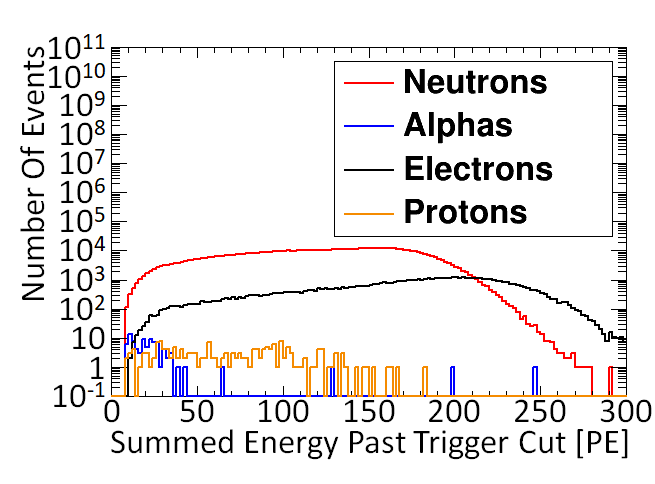
\includegraphics[width=\linewidth]{Chapter4.5/Figs/summedEnergyPastTrigLogAdjust.png}
  \captionof{figure}[Summed energy of neutron events that survive above the emulated trigger.]{The summed energy of the neutron events that survive above the emulated trigger. The simulated neutron trigger shown in figure \ref{fig:signalAndNoiseNeutronSVM_C1e6_g1e-6}. Efficiency = 75.3\,\% and purity = 91.7\,\%. Both are determined from a background of 4 million noise events and 1 million signal (neutron) events.} 
  \label{fig:summedEnergyPastTriggerGdDicebox}
    \vspace{1.434cm} %1 line = 0.478cm % 2 lines = 0.956cm % 3 lines= 1.434cm % 4 lines = 1.912cm % 5 lines = 2.39cm
\end{minipage}%
\qquad
\begin{minipage}{.45\textwidth}
  \centering
  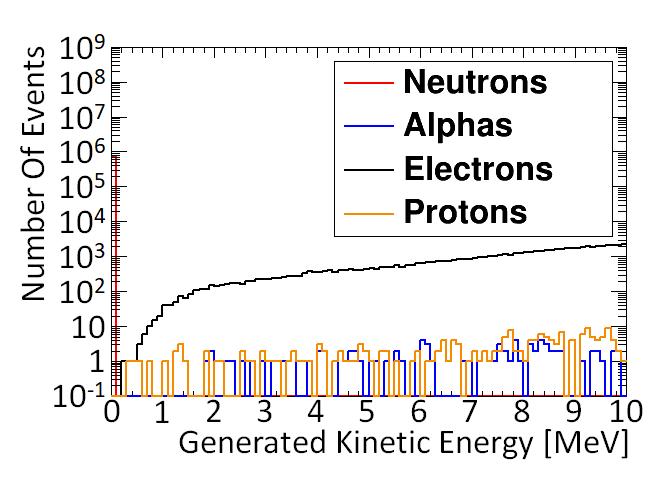
\includegraphics[width=\linewidth]{Chapter4.5/Figs/kineticEnergyPastTrigLogAdjust.png}
  \captionof{figure}[Generated kinetic energy for particles which make it above the emulated neutron trigger.]{The generated kinetic energy for particles which make it above the simulated neutron trigger. The only particles of concern are electrons that produce high enough energy to hit many bars and produce showers. Background electrons with energies > $\sim$4\,MeV are unlikely to be prevalent during deployment. Simulated neutron kinetic energies were 0.025\,eV. The 0$^\textrm{th}$ neutron bin goes up to $\sim 7.5 \times 10^5$.}
  \label{fig:GeneratedEnergyPastTriggerGdDicebox}
\end{minipage}
\end{figure}

\begin{table*}[!h]
\centering
\begin{tabular}{lccc}  
\toprule
Selection Criteria & \# of Dimensions & Efficiency\,[\%] & Purity\,[\%] \\
\midrule
manual            & 3                & 59.8             & 95.5         \\
SVM (Bars Only)    & 2                & 75.3             & 91.7         \\
SVM (Optimal)      & 2                & 78.6             & 94.8         \\
\bottomrule  
\end{tabular}
\caption{A comparison of the manual selection criteria and 2d SVMs with the bars only (NBATh$_{2.5}$ + NBATh$_{12.5}$) and the optimal (NBATh$_{2.5}$ + SEATh$_{2.5}$). The SVMs are able to improve upon the manual cuts significantly using 1 fewer dimension. Letting 15.5\,\% -- 18.8\,\% more neutrons through (thus improving efficiency) whilst reducing purity by 0.7\,\% -- 3.8\,\% which is an acceptable trade off.}
\label{tab:svmSelection}
\end{table*}

Finally, we can double check that the SVM boundary is sensible. In figure \ref{fig:signalAndNoiseNeutronSVM_C1e6_g1e-6} the SVM determines the events which are noise by excluding the events which have NBATh$_{12.5}\leq 6$ (low energy hits) and NBATh$_{2.5} \leq 5$ bar hits (small events). This is as expected as the DANCE-final state hybrid model has a greater chance of producing a cascade with high multiplicity (a large event) or low multiplicity with higher energy gamma-ray, (high energy hits). The loss in efficiency is therefore not concerning as low energy small events are atypical of the Gd cascade and will always be difficult to distinguish from noise. Fortunately the highly penetrating nature of the cascade gamma-rays means that even if the neutron is absorbed at the edge of the detector a large number of bars will be hit as the cascade will often extend to the edge of the detector. 
\\\\However, whilst the RBF SVM has proven to be effective at separating the Gd cascade from noise it's prudent to test other algorithms and compare their responses. A good way to do this is to compare their receiver operating characteristic (ROC) curves. This is specifically designed to compare the false positive rate to the true positive rate as the conditions change. In figure \ref{fig:rocCurvesKnnBdtSvm} the ROC curves for KNN (a,b), AdaBoosted DT (BDT) (c,d), linear SVM (e,f), RBF SVM (g,h) are all listed with a, c, e, g showing the optimum combination (NBATh$_{2.5}$, SEATh$_{2.5}$) and b, d, f, h showing bars only (NBATh$_{2.5}$, NBATh$_{12.5}$). All of these algorithm perform very well and have high accuracies, although the bars only KNN (figure \ref{subFig:knnBarsOnlyRoc}) seems to struggle its accuracy is still within 0.6\,\% of the other classifiers. The strong performance of each classifier can be seen in the incredible steepness of each ROC curve. This indicates that each classifier is able to separate the majority of true positives from false positives very well. However, the sudden shallowness of each ROC curve indicates that there is a small portion of the data with significant overlap between signal and noise. These results corroborate the C and $\gamma$ grid search (figure \ref{fig:GammaCGridSearchNeutron}). It can be concluded that any of the four machine learning classifiers would have been sufficient at separating the trigger data. Despite this training the RBF SVM classifier was still useful as much information was gained through observing its C and $\gamma$ grid search (i.e a small overlap in trigger data \& large degree of linearity in the trigger data). Also, as the SVM is convexly optimised (only 1 minimum) it is certain that the classifier has not optimised for a local minimum and has found an accurate, generalised solution. 
\begin{figure}[!h]
\centering
\begin{subfigure}{.4\textwidth}
  \centering
  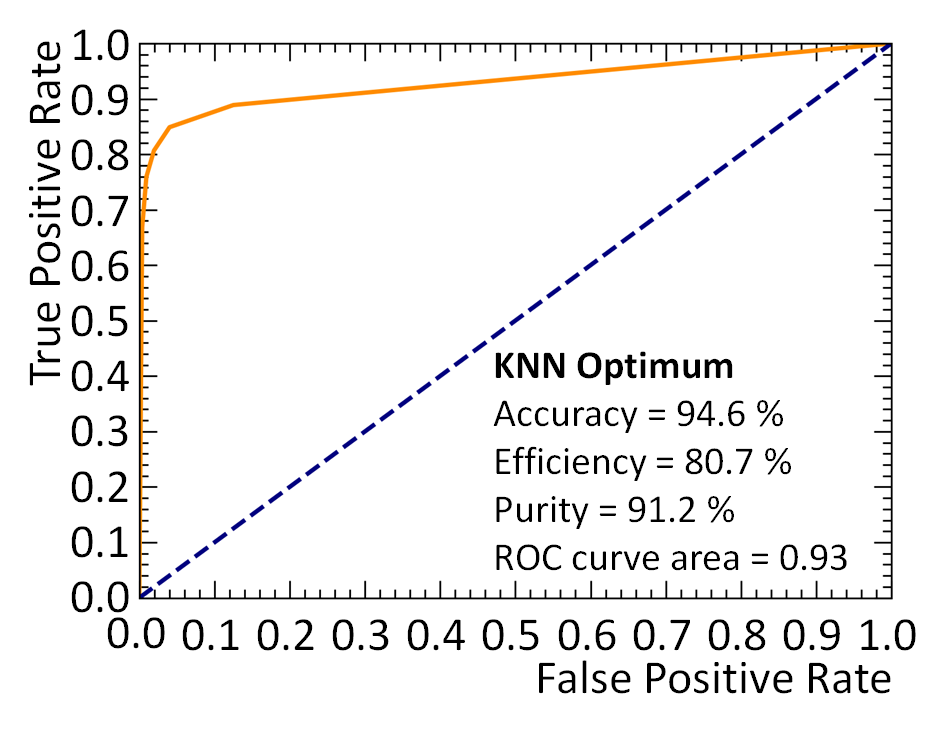
\includegraphics[width=\linewidth]{Chapter4.5/Figs/knnOptimumRoc.png}
  \captionsetup{width=.9\linewidth}
  \caption{}
  \label{subFig:knnOptimumRoc}
\end{subfigure}%
\qquad
\begin{subfigure}{.4\textwidth}
  \centering
  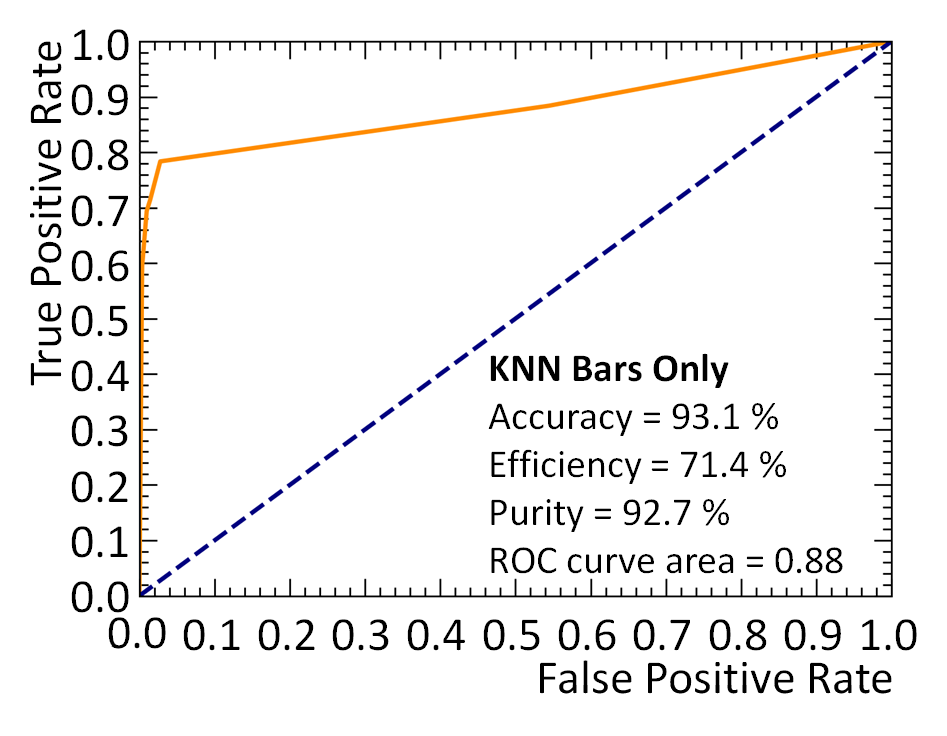
\includegraphics[width=\linewidth]{Chapter4.5/Figs/knnBarsOnlyRoc.png}
  \captionsetup{width=.9\linewidth}
  \caption{}
  \label{subFig:knnBarsOnlyRoc}
\end{subfigure}
\begin{subfigure}{.4\textwidth}
  \centering
  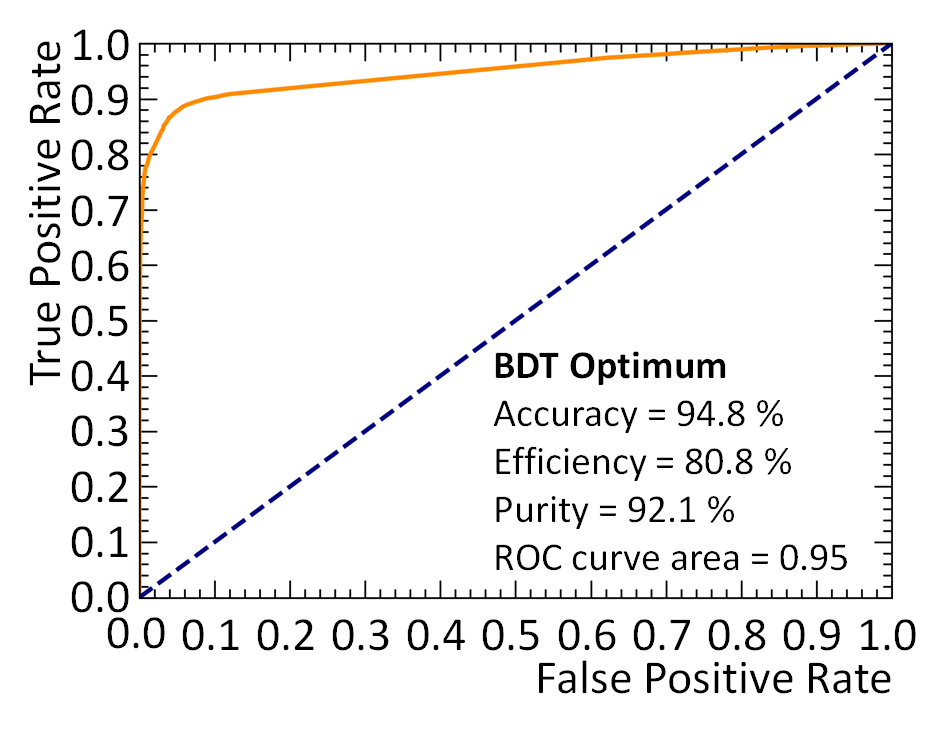
\includegraphics[width=\linewidth]{Chapter4.5/Figs/bdtOptimumRoc.png}
  \captionsetup{width=.9\linewidth}
  \caption{}
  \label{subFig:bdtOptimumRoc}
\end{subfigure}
\qquad
\begin{subfigure}{.4\textwidth}
  \centering
  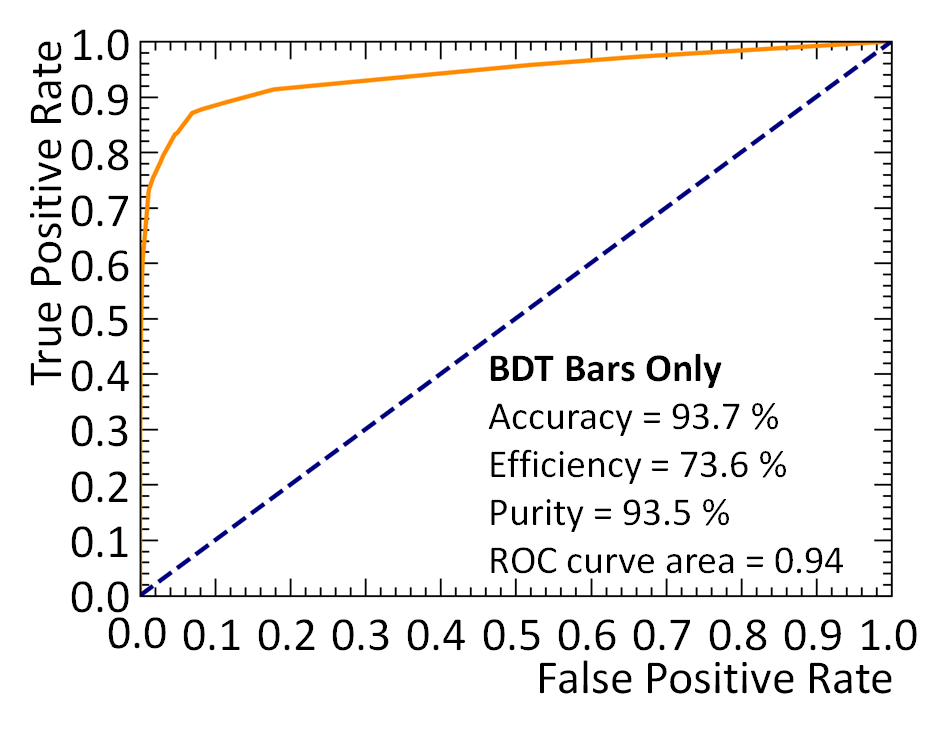
\includegraphics[width=\linewidth]{Chapter4.5/Figs/bdtBarsOnlyRoc.png}
  \captionsetup{width=.9\linewidth}
  \caption{}
  \label{subFig:bdtBarsOnlyRoc}
\end{subfigure}
\begin{subfigure}{.4\textwidth}
  \centering
  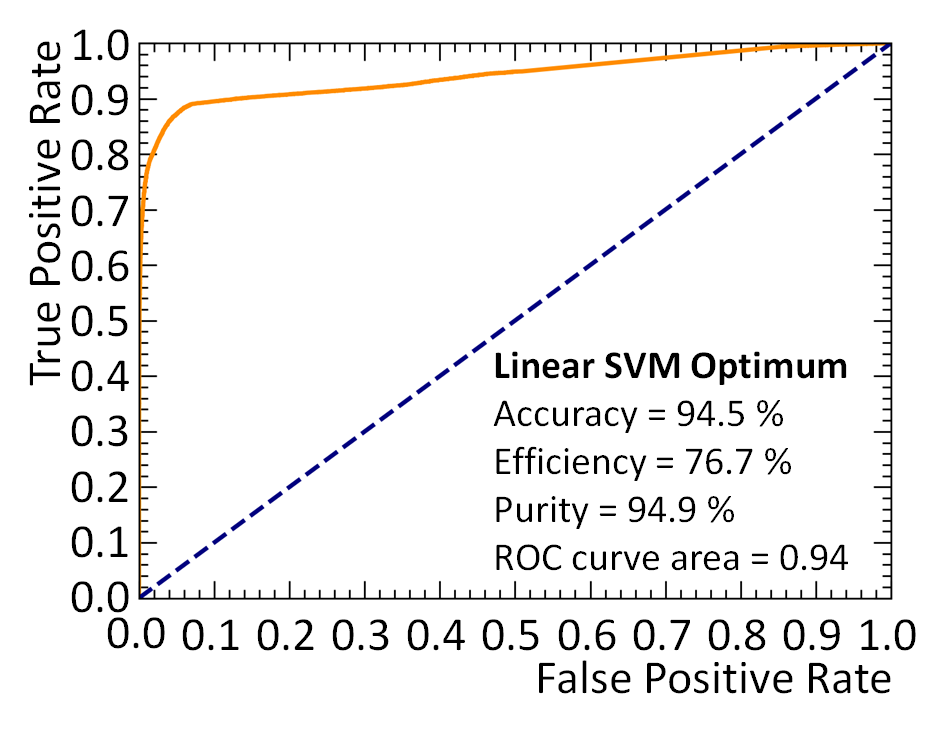
\includegraphics[width=\linewidth]{Chapter4.5/Figs/linSvmOptimumRoc.png}
  \captionsetup{width=.9\linewidth}
  \caption{}
  \label{subFig:linSvmOptimumRoc}
\end{subfigure}
\qquad
\begin{subfigure}{.4\textwidth}
  \centering
  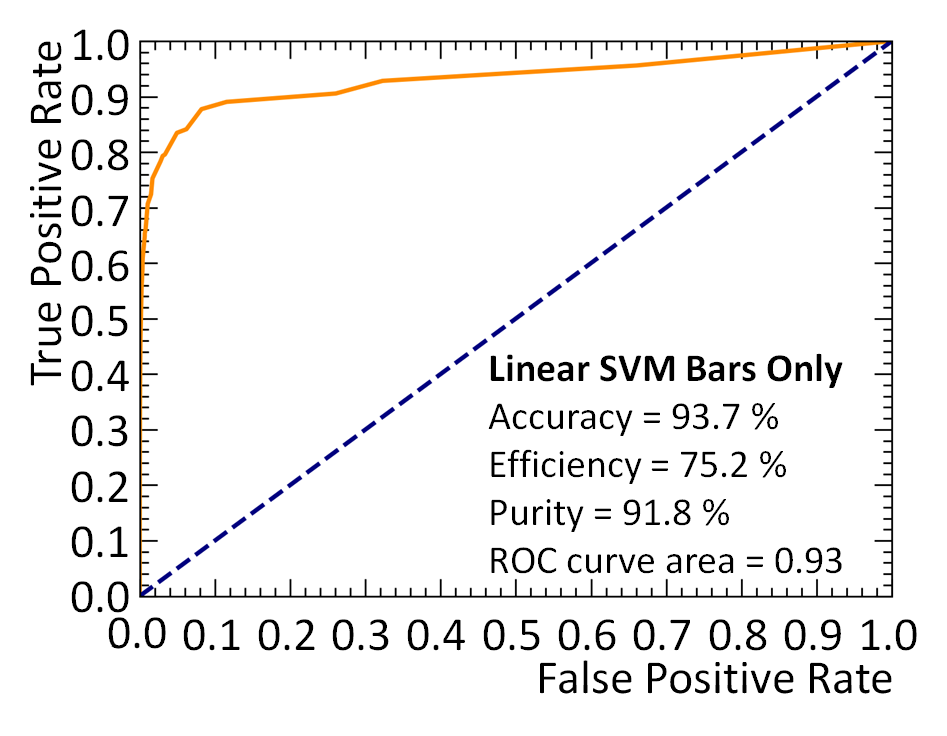
\includegraphics[width=\linewidth]{Chapter4.5/Figs/linSvmBarsOnlyRoc.png}
  \captionsetup{width=.9\linewidth}
  \caption{}
  \label{subFig:}
\end{subfigure}
\begin{subfigure}{.4\textwidth}
  \centering
  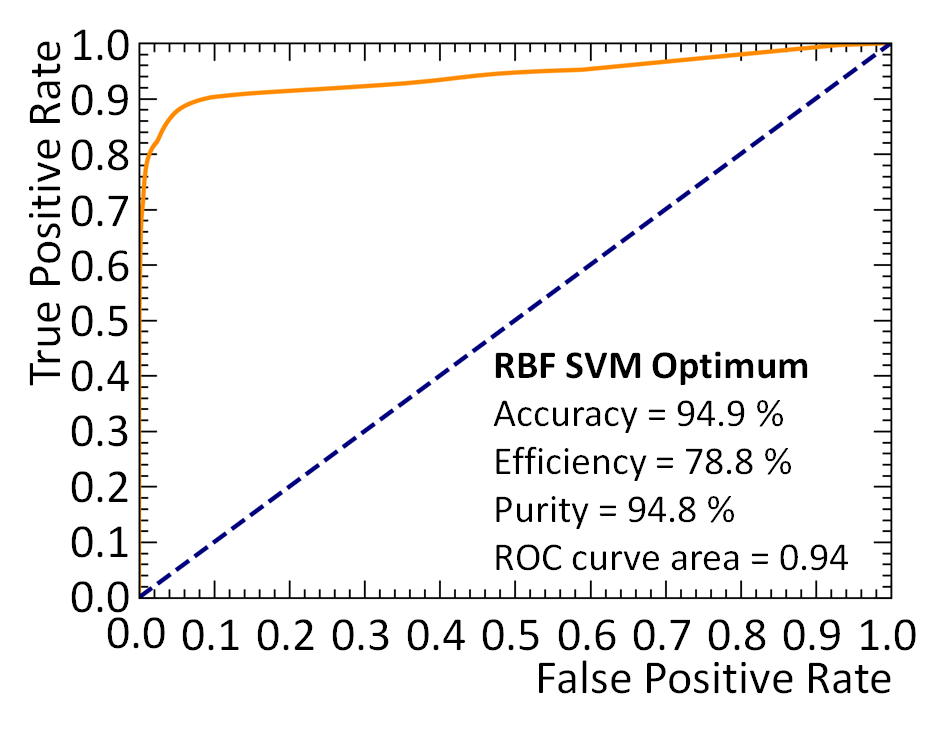
\includegraphics[width=\linewidth]{Chapter4.5/Figs/rbfSvmOptimumRoc.png}
  \captionsetup{width=.9\linewidth}
  \caption{}
  \label{subFig:linSvmBarsOnlyRoc}
\end{subfigure}
\qquad
\begin{subfigure}{.4\textwidth}
  \centering
  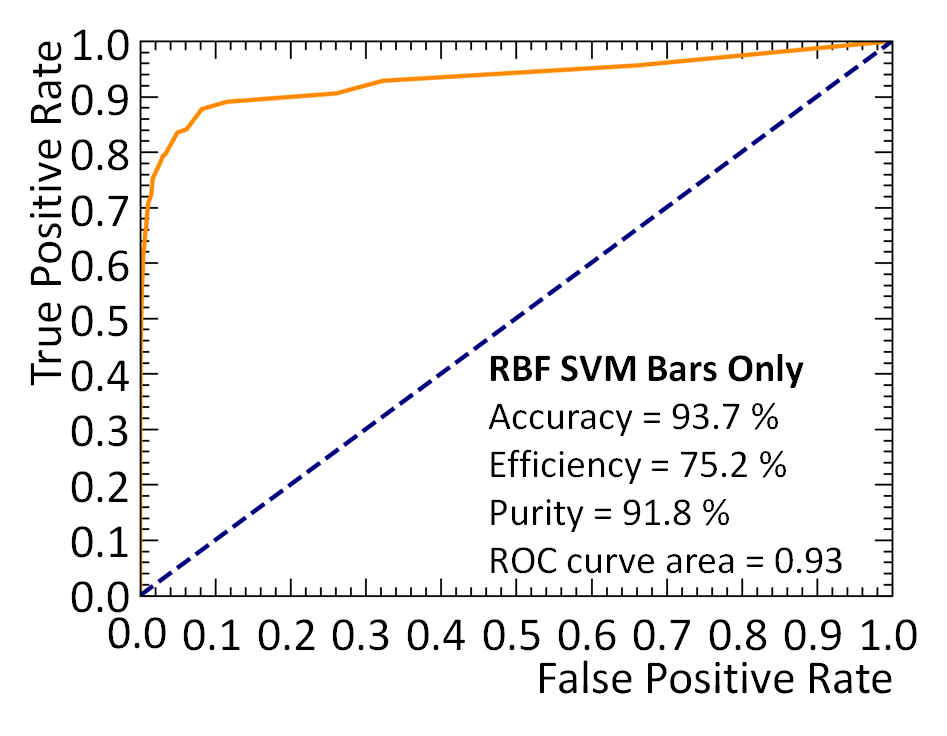
\includegraphics[width=\linewidth]{Chapter4.5/Figs/rbfSvmBarsOnlyRoc.png}
  \captionsetup{width=.9\linewidth}
  \caption{}
  \label{subFig:rbfSvmBarsOnlyRoc}
\end{subfigure}
\caption[ROC curves for KNN, AdaBoosted DT (BDT), linear SVM, and RBF SVM on optimum and bars only trigger data.]{ROC curves for KNN, AdaBoosted DT (BDT), linear SVM, and RBF SVM on optimum and bars only trigger data, labelled accordingly. The KNN appears to be the weakest classifier whilst the BDT, Linear SVM and RBF SVM agree strongly with each other. The classifier with the highest accuracy is the RBF SVM optimum, but each classifier separates the data well as its 2d largely linearly separable data.}
\label{fig:rocCurvesKnnBdtSvm}
\end{figure}

\clearpage
\section{Modelling Muons}
Muons are highly penetrating high energy particles. As a result atmospheric muons act as minimally ionising particles (MIPs) and the amount of energy deposited per cm ($dE/dx$) is largely independent of the generated energy for the range of 100\,MeV/$c$ -- 100\,GeV/$c$ (see figure \ref{fig:pdg_MuonMomentumStopping}). Whilst figure \ref{fig:pdg_MuonMomentumStopping} shows many different effects and when they take effect for muons this figure only shows the effect incident on a copper surface. The detector is not comprised of Cu it is comprised of hydrocarbons, specifically polystyrene. By mass polystyrene is more C than H so by looking at the momentum ranges 0.1\,GeV/$c$ to 100\,GeV/$c$ in figure \ref{fig:pdg_dedx_gcm2}, it is reasonable to assume a dE/dx of $\sim$ 2 g$^{-1}$ cm$^2$ for muons on C. The advantage of nearly all cosmic muons having a similar response in plastic scintillator means that the are extremely useful for detector energy calibration. 

\begin{figure}[!h]
 \centering
 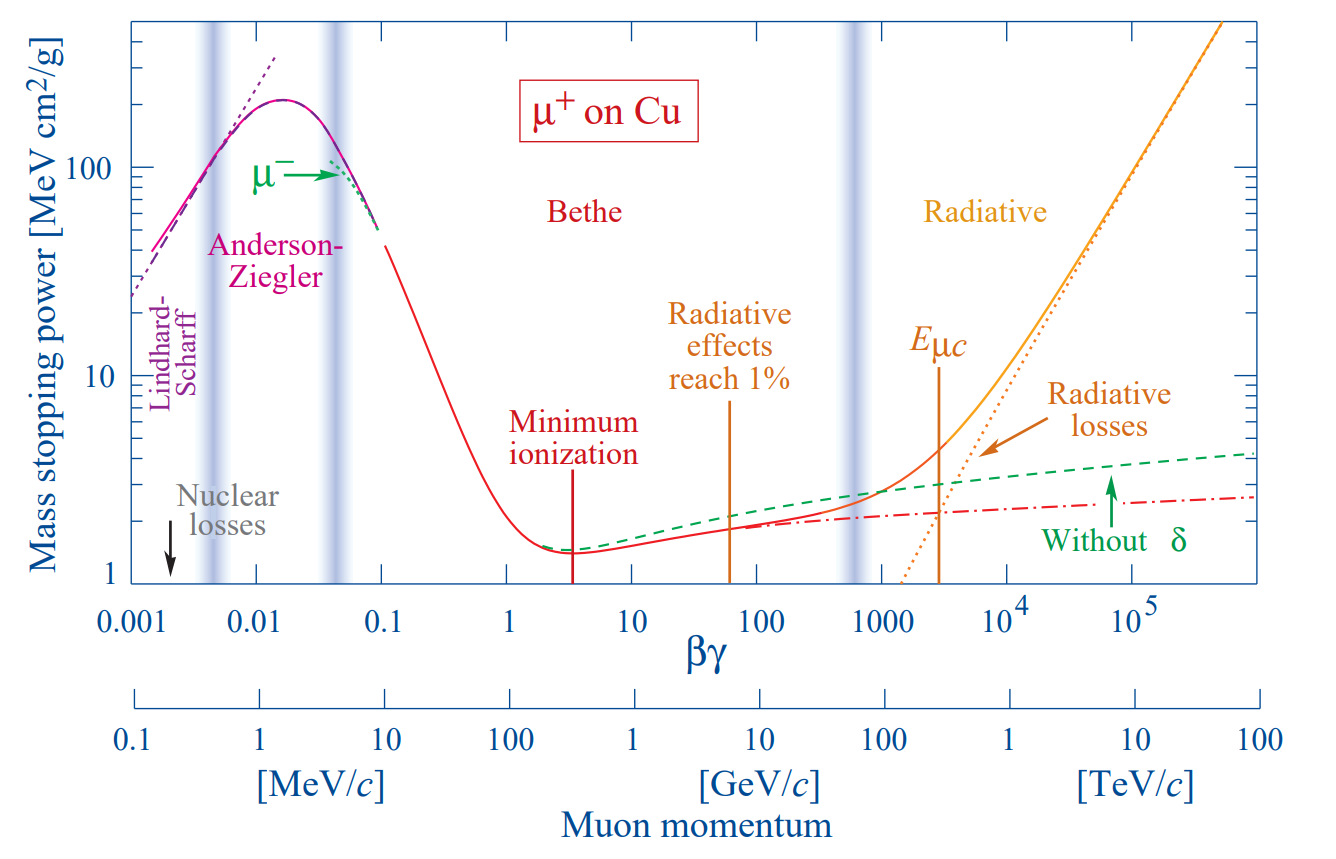
\includegraphics[width=0.7\linewidth]{Chapter4/Figs/Raster/pdg_MuonMomentumStopping.png}
 \captionof{figure}[Mass stopping power for positive muons in copper.]{Mass stopping power for positive muons in copper as a function of $\beta \gamma$ = $\rho/Mc$ over nine orders of magnitude in momentum (12 orders of magnitude in kinetic energy). From \cite{Olive_2014}.} 
 \label{fig:pdg_MuonMomentumStopping}
\end{figure}

\begin{figure}[!h]
 \centering
 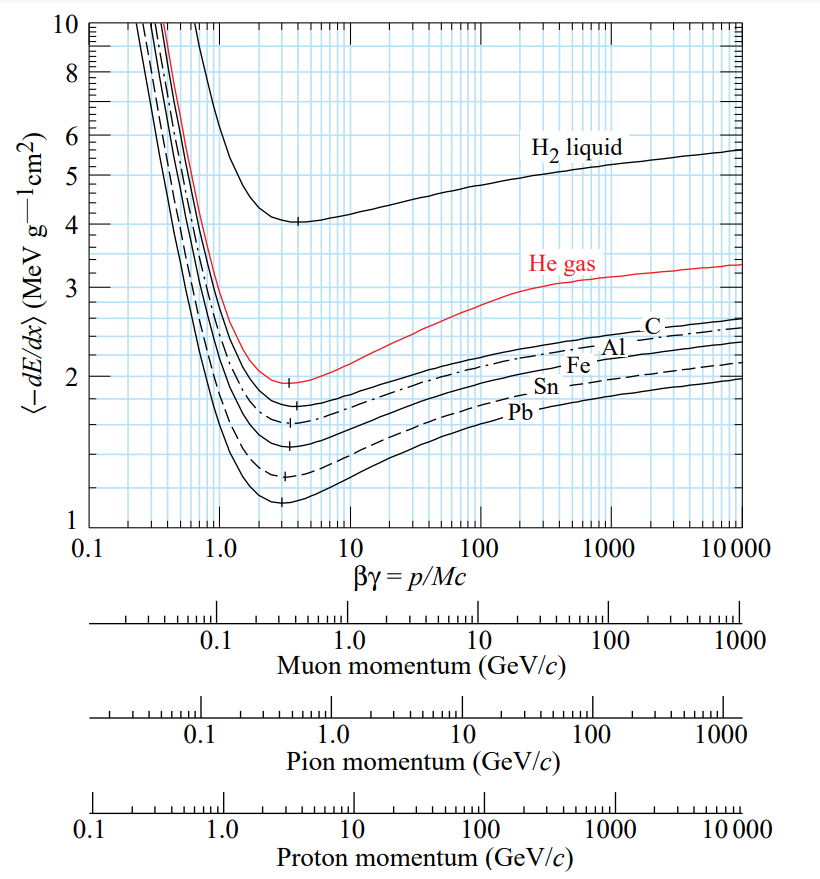
\includegraphics[width=0.7\linewidth]{Chapter4/Figs/Raster/pdg_dedx_gcm2.png}
 \captionof{figure}[Mean energy loss rate in liquid (bubble chamber) for muons.]{Mean energy loss rate in liquid (bubble chamber) hydrogen, gaseous helium, carbon, aluminium, iron, tin, and lead. Radiative effects, relevant for
muons and $\pi$, are not included. From \cite{Olive_2014}.} 
 \label{fig:pdg_dedx_gcm2}
\end{figure}

By simulating a single scintillating bar of dimensions $4\,\textrm{cm} \times 152\,\textrm{cm} \times 1\,\textrm{cm}$ (x,y,z) and firing a muon directly down in the z-plane (figure \ref{fig:lengthAndSideViewBarMuon}) it is possible to determine the $dE/dx$ in simulation. The energy deposition approximates $dE/dx$ in units of MeV/cm. By simulating kinetic muon energies from 0.1\,MeV -- 250\,MeV in figure \ref{fig:muon_0_250} the mean energy deposition settles to MIP levels of $\sim$ 2 MeV/cm between 100\,MeV -- 200\,MeV. The CRY library \cite{ieee_cry_2007} can then be used to approximate the expected energies from cosmic muons which is shown in figure \ref{fig:keMevCryMuons}. In figure \ref{fig:keMevCryMuons} over 99\,\% of the muon particles produced by the CRY library are between 0.1\,GeV -- 40\,GeV. This coupled with figures \ref{fig:pdg_MuonMomentumStopping} and \ref{fig:pdg_dedx_gcm2} make it reasonable to assume that over 99\,\% of the expected muon distribution will be MIP-like in its behaviour. The distribution for the energy loss of fast particles by ionisation was quantified by Landau in 1944 \cite{landau1944energy}. The Landau distribution represents the energy deposited and is characterised by a sharp peak with a long tail. When simulating high energy muons this Landau distribution is visible in the events that deposit in the bar shown by figure \ref{fig:mev_per_cm_muons}. Using the points previously discussed it is reasonable to assume that over 99\,\% of events will follow a Landau distribution. %and can be seen in the simulated bar results in figure \ref{fig:mev_per_cm_muons}. More than 99\,\% of the muons$ distribution will have the Landau distribution shown in figure \ref{fig:mev_per_cm_muons}. 

\begin{figure}[!h]
\centering
\begin{minipage}{.45\textwidth}
  \centering
  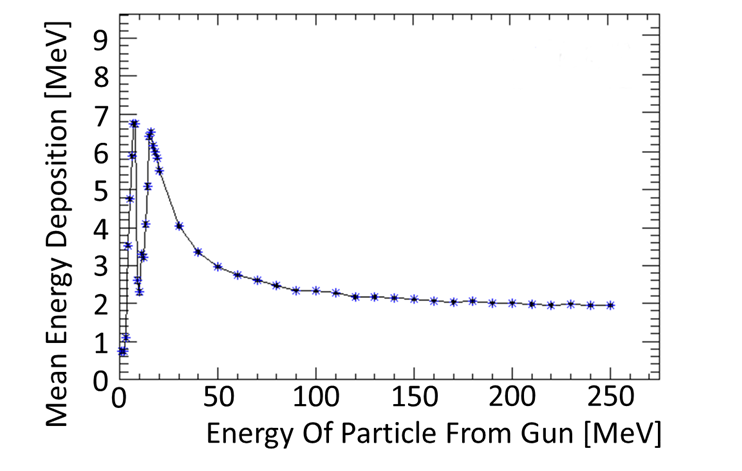
\includegraphics[width=\linewidth]{Chapter4/Figs/Raster/Muon_TiO2_med_engMedText.png}
  \captionof{figure}[Muon mean energy deposition in the active component of the single bar.]{Muon mean energy deposition in the active component of the single bar, the sharp decrease in the energy deposited and varying deposition below 20\,MeV was due to the TiO$_2$ coating absorbing muons at lower energies.} 
  \label{fig:muon_0_250}
  \vspace{0.956cm} %1 line = 0.478cm % 2 lines = 0.956cm % 3 lines= 1.434cm % 4 lines = 1.912cm % 5 lines = 2.39cm
\end{minipage}%
\qquad
\begin{minipage}{.45\textwidth}
  \centering
  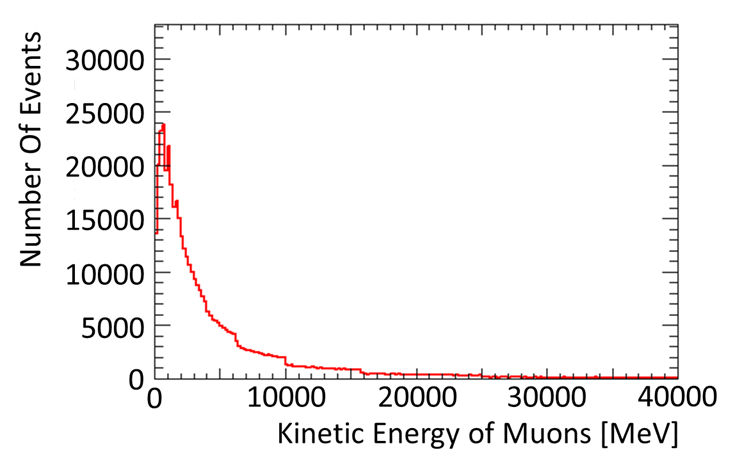
\includegraphics[width=\linewidth]{Chapter4/Figs/Raster/keMevCryMuonsMedText.png} 
  \captionof{figure}[Generated kinetic energy for muons using the CRY library at sea level.]{Generated kinetic energy for muons using the CRY library \cite{ieee_cry_2007} at sea level with latitude 53$^\circ$ (Liverpool and Wylfa's latitude) and date: 01 -- March -- 2021. 99\,\% + of generated muon particles are between 0.1\,GeV (100\,MeV) and 40\,GeV (40000\,MeV) kinetic energy.}
  \label{fig:keMevCryMuons}
\end{minipage}
\end{figure}

\begin{figure}[!h]
 \centering
 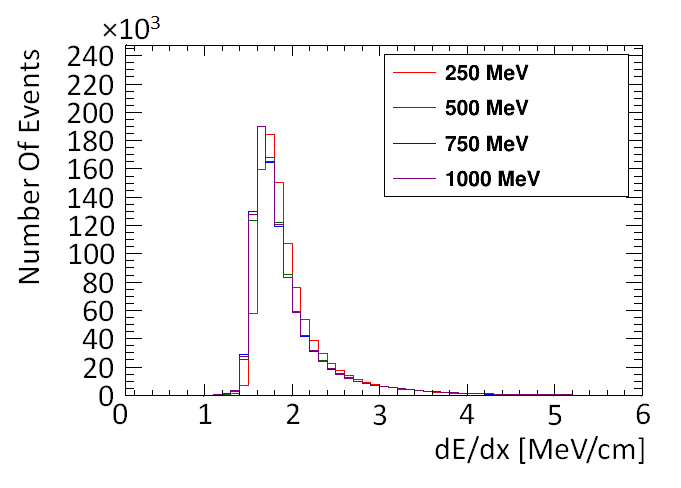
\includegraphics[width=0.5\linewidth]{Chapter4/Figs/Raster/year1Plots/muons_per_mev_cmMedText.png}
 \captionof{figure}[dE/dx of muons through single a plastic bar.]{dE/dx of muons through single a plastic bar assuming a density of plastic of 1\,g\,cm$^{-3}$. Measurements for plastic are similar to carbon. For carbon $\sim$ 2\,MeV\,cm$^{-1}$ is expected for dE/dx {\cite{Olive_2014}. Mean dE/dx for 250\,MeV, 500\,MeV, 750\,MeV, 1000\,MeV are respectively 1.9907 $\pm$  0.0005\,MeV\,cm$^{-1}$, 1.9387 $\pm$  0.0005\,MeV\,cm$^{-1}$, 1.9374 $\pm$  0.0005 MeV\,cm$^{-1}$, 1.9407 $\pm$  0.0005 MeV\,cm$^{-1}$.\\}}
 \label{fig:mev_per_cm_muons}
\end{figure}

As mentioned before the CRY library is very useful as it contains a large amount of relevant physics information with the latest version being 1.7 produced in 2012 \cite{hagmann2012cosmicCry}. The CRY library splits up the directions in the $x$,$y$ and $z$ by using cosine directions $u$ (see equation \ref{equ:cos_u}), $v$ (see equation \ref{equ:cos_v}) and $w$ (see equation \ref{equ:cos_w}) respectively, with $\cos(w) = \cos(\theta)$, where $\theta$ is the polar angle. However, whilst the generated cosine direction for $u$ and $v$ were very fine the binning for $\cos(\theta)$ was coarse. As a result, an 8$^{\textrm{th}}$ order polynomial function was fitted to the $\cos(\theta)$ distribution in figure \ref{fig:Cry_GeneratedFit} to smooth out the distribution. An 8$^{\textrm{th}}$ order polynomial is used to ensure that a function traversed all of the points in the $\cos{\theta}$ curve. 8$^{\textrm{th}}$ was the lowest order that achieved this. This is not strictly physical, however it is merely representing that for each generated $\cos(\theta)$ bin it is more likely that the bins next to it are better at interpolating the edges between bins. This is later compared to the measured $\theta$ results at Wylfa and Liverpool in section \ref{sec:usingSimulatedDataAsControlData} which it resembles more accurately with the smoothing than without. The improvement to the distribution can be seen in figure \ref{fig:CrySmoothingCosTheta} where the finer binning of the $\cos(\theta)$ in figure \ref{subFig:CrySmoothingCosine} leads to a smoother and more accurate $\theta$ distribution in figure \ref{subFig:CrySmoothingTheta}. 

\begin{equation}
\alpha = \cos{u} = \frac{v_x}{\sqrt{v_x^2+v_y^2+v_z^2}}
\label{equ:cos_u}
\end{equation}

\begin{equation}
\beta = \cos{v} = \frac{v_y}{\sqrt{v_x^2+v_y^2+v_z^2}}
\label{equ:cos_v}
\end{equation}

\begin{equation}
\gamma = \cos{w} = \frac{v_z}{\sqrt{v_x^2+v_y^2+v_z^2}}
\label{equ:cos_w}
\end{equation}

\begin{figure}[!h]
 \centering
 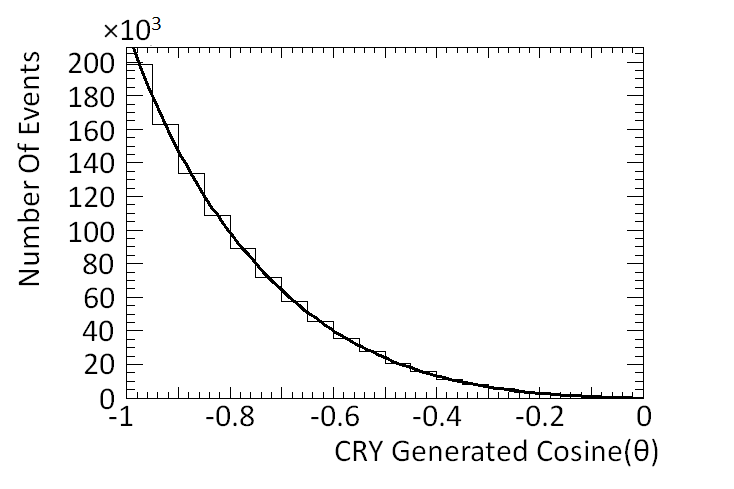
\includegraphics[width=0.5\linewidth]{Chapter4/Figs/CryFitCosWMedText.png}
 \captionof{figure}[Generated angles for cosine direction W from the CRY library.]{The generated angles for cosine direction W ($\cos(\theta)$) (z-axis) from the CRY library \cite{ieee_cry_2007} for 1 million particles. Binning in CRY is 0.05 so an 8-dimensional polynomial was fitted to smooth the distribution.}
 \label{fig:Cry_GeneratedFit}
\end{figure}

\begin{figure}[!h]
\centering
\begin{subfigure}{.5\textwidth}
  \centering
  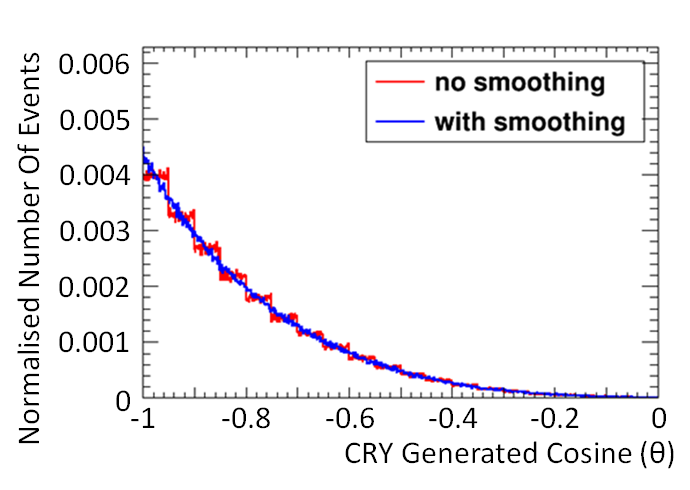
\includegraphics[width=\linewidth]{Chapter4/Figs/Raster/CryPlots/CrySmoothingCosineMedText.png}
  \captionsetup{width=.9\linewidth}
  \caption{}
  \label{subFig:CrySmoothingCosine}
\end{subfigure}%
\begin{subfigure}{.5\textwidth}
  \centering
  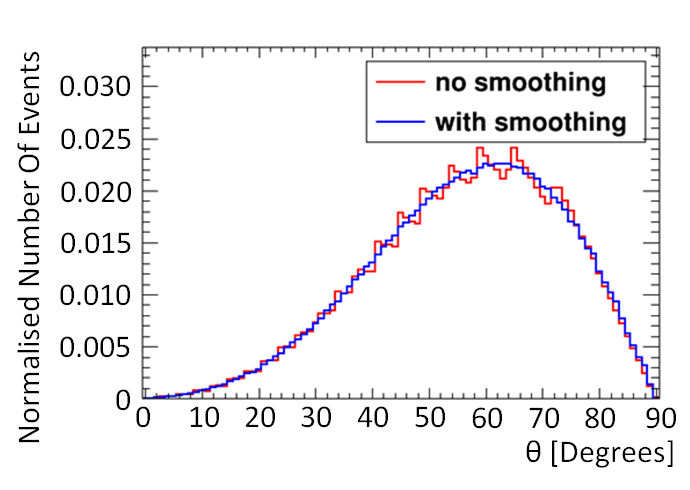
\includegraphics[width=\linewidth]{Chapter4/Figs/Raster/CryPlots/CrySmoothingThetaMedText.png}
  \captionsetup{width=.9\linewidth}
  \caption{}
  \label{subFig:CrySmoothingTheta}
\end{subfigure}
\caption[How the 8$^\textrm{th}$ order polynomial smoothing affects the CRY distribution in $\cos{w}$.]{How the 8$^\textrm{th}$ order polynomial smoothing affects the CRY distribution in $\cos{w}$ ($\cos{\theta}$) (see (a)) and $\theta$ (see (b)). The nonphysical peaks seen in the non-smoothed $\theta$ distribution are a direct result of CRY's coarse binning in $\cos{\theta}$.}
\label{fig:CrySmoothingCosTheta}
\end{figure}

Now the $\theta$ distribution has been smoothed out the cosmic muon particles need to be back-projected. Back projection is where positions that CRY generates (see figure \ref{fig:cryxm_vs_cryym}) are taken as a ``target'' and then the $\phi$ values (a flat distribution between 0 -- 360$^\circ$) and smoothed $\theta$ values (see figure \ref{subFig:CrySmoothingTheta}) are used to project backwards find a start vertex for a given radius. The larger the back projection radius, the more accurate the simulation but the more computationally intensive it becomes. A back-projection of 100\,m is a reasonable approximation to simulate all incoming side-on and top-down events. Figure \ref{fig:BackProjectionXY} shows the top-down ($x$,$y$) distribution when back projecting by 100\,m. The ``halo'' in figure \ref{fig:BackProjectionXY} is a result of the $\theta$ distribution seen in figure \ref{subFig:CrySmoothingTheta}. The rest of the simulated dome can be seen in figure \ref{fig:BackProjection_XZ_YZ} where the ($x$,$z$) and ($y$,$z$) distributions are very similar to each other. 


\begin{figure}[!h]
\centering
\begin{minipage}{.45\textwidth}
  \centering
  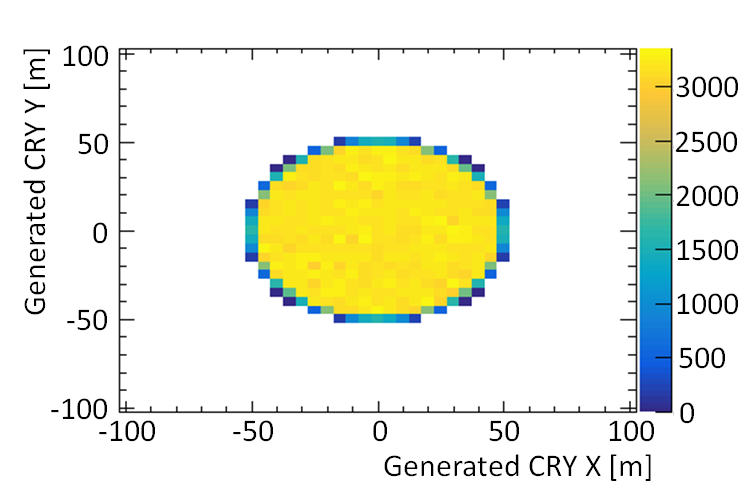
\includegraphics[width=\linewidth]{Chapter4/Figs/Raster/CryPlots/cryxm_vs_cryymMedText.png}
  \captionof{figure}[Generated CRY (x,y) positions in simulation.]{Generated CRY (x,y) positions in the simulation. A circle has been cut out of the generated square to give a flat $\phi$ distribution. All particles in CRY are generated at Z = 0.} 
  \label{fig:cryxm_vs_cryym}
\end{minipage}%
\qquad
\begin{minipage}{.45\textwidth}
  \centering
  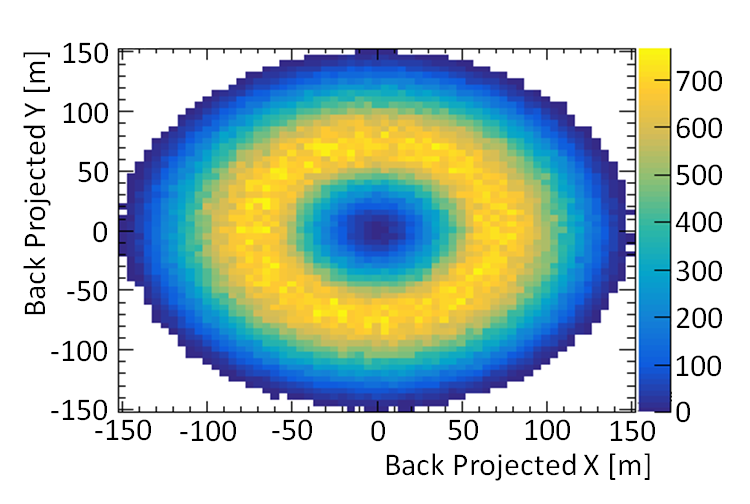
\includegraphics[width=\linewidth]{Chapter4/Figs/Raster/CryPlots/BackProjectionXYMedText.png} 
  \captionof{figure}[Back projection of 100\,m in the (x,y) plane for the CRY library.]{Back projection of 100\,m in the (x,y) plane for the CRY library this represents the starting vertex for each particle generated in (x,y).}
  \label{fig:BackProjectionXY}
\end{minipage}
\end{figure}

\begin{figure}[!h]
\centering
\begin{subfigure}{.5\textwidth}
  \centering
  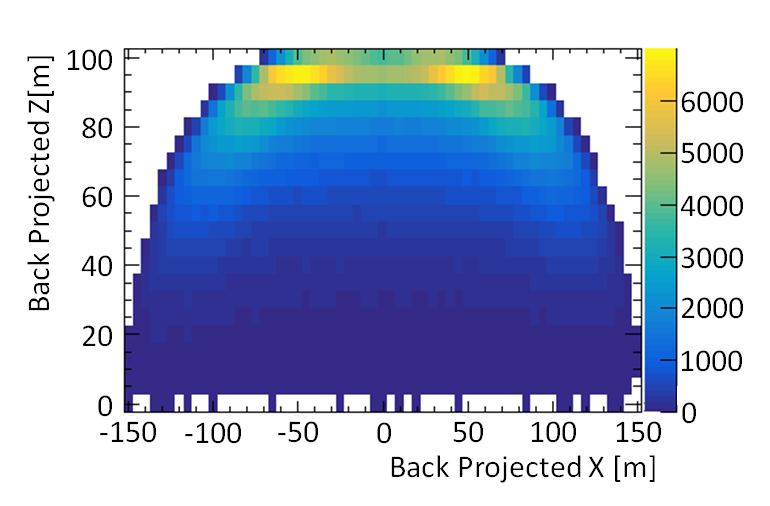
\includegraphics[width=\linewidth]{Chapter4/Figs/Raster/CryPlots/BackProjectionXZMedText.png}
  \captionsetup{width=.9\linewidth}
  \caption{}
  \label{subFig:BackProjectionXZ}
\end{subfigure}%
\begin{subfigure}{.5\textwidth}
  \centering
  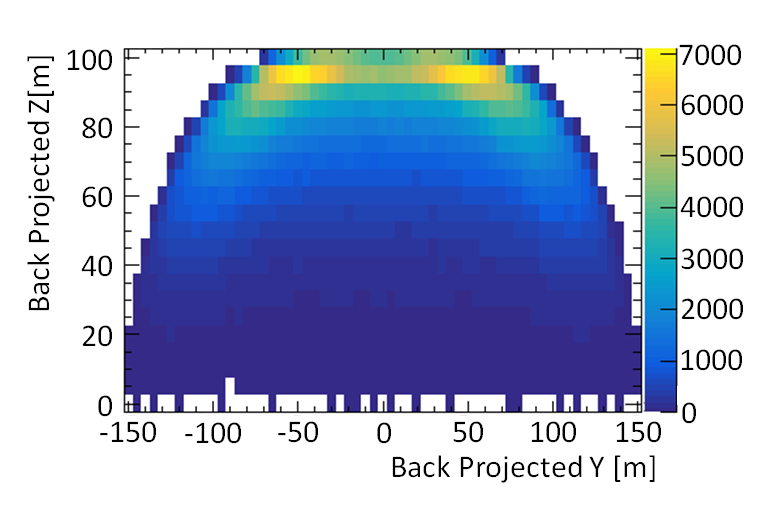
\includegraphics[width=\linewidth]{Chapter4/Figs/Raster/CryPlots/BackProjectionYZMedText.png}
  \captionsetup{width=.9\linewidth}
  \caption{}
  \label{subFig:BackProjectionYZ}
\end{subfigure}
\caption[Starting positions for the generated CRY distribution.]{Starting positions for the generated CRY distribution for (x,z) (see (a)) and (y,z) (see (b)) with a back projection of 100\,m.}
\label{fig:BackProjection_XZ_YZ}
\end{figure}

The impact of back-projection is relatively small when looking at where the particles cross the $z$-axis. As shown in figure \ref{fig:Crossed_atZ_XY_AndShort} when comparing a back projection of 0.01\,m (figure \ref{subFig:CrossedZAxisShort}) to 100\,m (figure \ref{subFig:Crossed_atZ_XY}) both reproduce the circular distribution seen in figure \ref{fig:cryxm_vs_cryym}. There is more scattering with more back-projection but this is a suitable trade-off for vastly more accurate tracks. 

\begin{figure}[!h]
\centering
\begin{subfigure}{.5\textwidth}
  \centering
  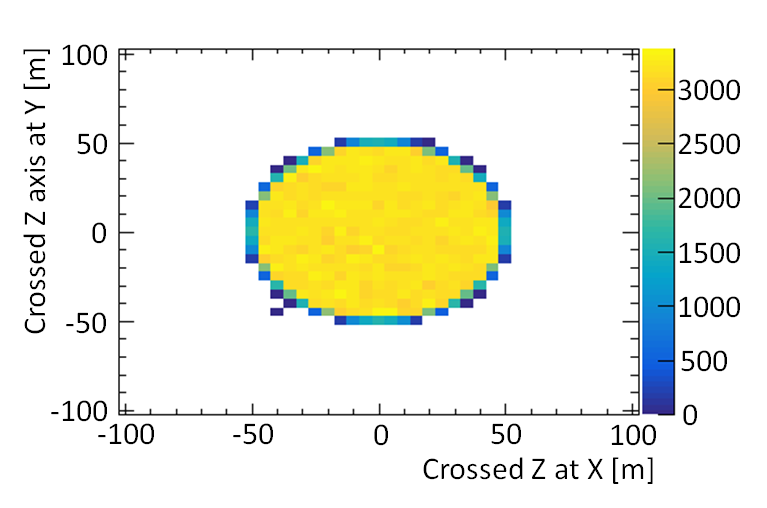
\includegraphics[width=\linewidth]{Chapter4/Figs/Raster/CryPlots/CrossedZAxisShortMedText.png}
  \captionsetup{width=.9\linewidth}
  \caption{}
  \label{subFig:CrossedZAxisShort}
\end{subfigure}%
\begin{subfigure}{.5\textwidth}
  \centering
  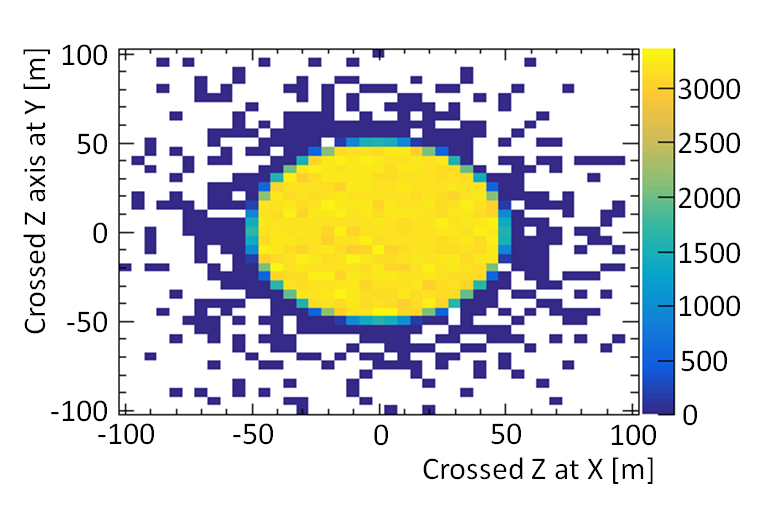
\includegraphics[width=\linewidth]{Chapter4/Figs/Raster/CryPlots/Crossed_atZ_XYMedText.png}
  \captionsetup{width=.9\linewidth}
  \caption{}
  \label{subFig:Crossed_atZ_XY}
\end{subfigure}
\caption[How the generated CRY distribution crosses the Z-axis.]{How the generated CRY distribution crosses the Z-axis with only 1\,cm of back-projection (see (a)) vs 100\,m of back projection (see (b)). When the GEANT4 environment emulates the vacuum of space.}
\label{fig:Crossed_atZ_XY_AndShort}
\end{figure}

In addition, atmospheric effects need to be modelled. The atmosphere impacts the cosmic muon distribution in two main ways: it increases particle scattering (see figure \ref{fig:gen-scat_PhiTheta}) and the rate of secondaries produced (see figure \ref{fig:CRY_rates}). The CRY simulation takes the atmosphere into account \cite{hagmann2007monteCry} but only produces the particles that cross the $z$-axis at $z = 0$. As a result the secondaries produced by GEANT4 are also simulated by CRY thus resulting in some secondary particles being ``double simulated.'' This effect is most visible in figure \ref{fig:CRY_rates} where the rates in simulated air are overall $\sim$ 25\,\% higher than in \texttt{G4$\textunderscore$Galactic} (an environment in GEANT4 designed to emulate the vacuum of space). However, the paths of these particles are more accurate in air and the secondaries produced inside a detector still need to be taken into account. For the most accurate cosmic modelling, air should be used whilst removing all secondaries that occur in the air i.e outside the detector. However, due to time constraints atmospheric scattering without ``double simulated'' secondaries was unable to be added to the simulation. 

\begin{figure}[!h]
\centering
\begin{subfigure}{.5\textwidth}
  \centering
  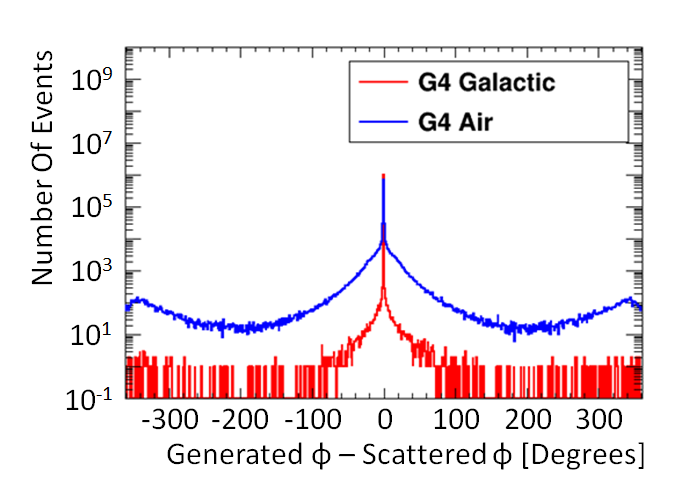
\includegraphics[width=\linewidth]{Chapter4/Figs/Raster/CryPlots/genPhi-scatPhiMedText.png}
  \captionsetup{width=.9\linewidth}
  \caption{}
  \label{subFig:genPhi-scatPhi}
\end{subfigure}%
\begin{subfigure}{.5\textwidth}
  \centering
  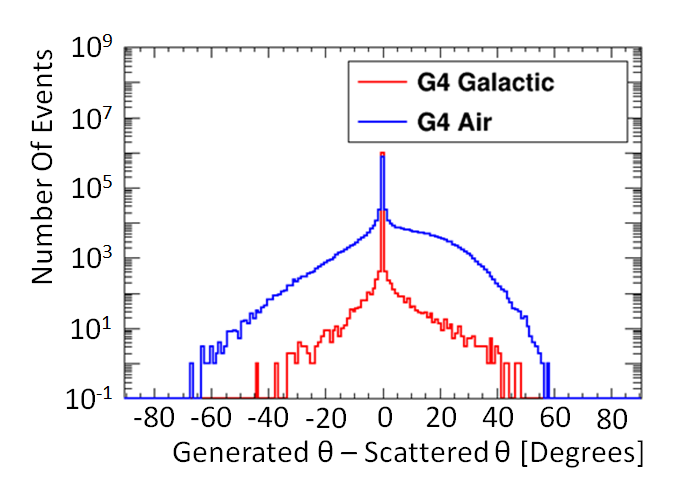
\includegraphics[width=\linewidth]{Chapter4/Figs/Raster/CryPlots/genTheta-scatThetaMedText.png}
  \captionsetup{width=.9\linewidth}
  \caption{}
  \label{subFig:genTheta-scatPhi}
\end{subfigure}
\caption[Difference between generated and scattered angular direction in GEANT4.]{Difference between generated and scattered angular direction in GEANT4 in $\theta$ (a) and $\phi$ (b).}
\label{fig:gen-scat_PhiTheta}
\end{figure}

\begin{figure}[!h]
 \centering
 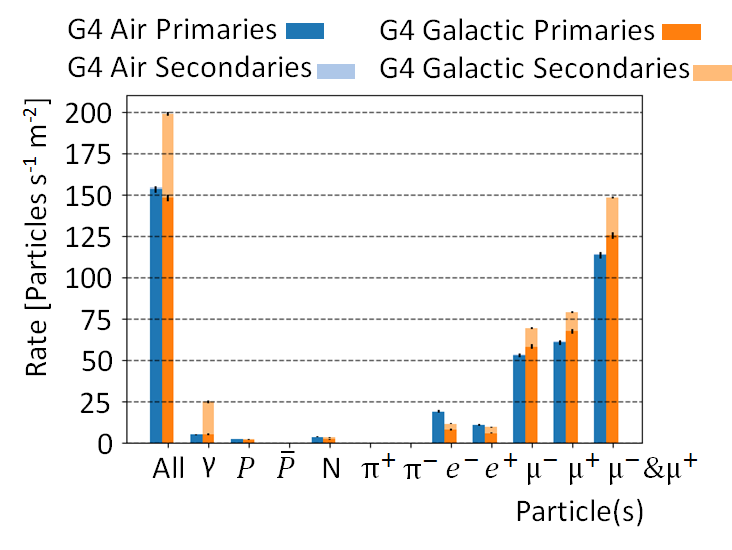
\includegraphics[width=0.7\linewidth]{Chapter4/Figs/Raster/CryPlots/CRY_ratesMedText.png}
 \captionof{figure}[Rate dependence on the world material in GEANT4.]{Rate dependence on the world material in GEANT4. For \texttt{G4$\textunderscore$Galactic} world materials, secondary production is minimal. The rates are most accurate for Galactic world material but the paths will be more accurate for \texttt{G4$\textunderscore$Air}. Simulated in a PVT block of 1\,m $\times$ 1\,m $\times$ 1\,cm to approximate particles s$^{-1}$ m$^{-2}$.} 
 \label{fig:CRY_rates}
\end{figure}

In conclusion, muon modelling is important as for above-ground reactor operation they are a key aspect of background due to their highly penetrating nature and high incident rate. However, the MIP-like nature of these particles makes them ideal for calibration as their response is consistent ($\sim$ 2\,MeV/cm). In addition, modelling the muon distribution with CRY \cite{ieee_cry_2007} allows for a more accurate $\theta$ distribution. The large energy and highly penetrating nature of cosmic muons means they create large discernible tracks in the detector. These tracks hit many bars as they traverse through the detector and so the $\phi$ and $\theta$ can be reliably reconstructed. This track reconstruction could therefore be used for tomographic purposes. As a result, it should be possible to use this simulated distribution as a control data set for cosmic muon tomography which is done in section \ref{sec:usingSimulatedDataAsControlData} when attempting to highlight cosmic muon deficits caused by buildings. This is done whilst ensuring that \texttt{G4$\textunderscore$Air} is simulated in the world to ensure a more accurate scattering model. 

\section{Muon Tracker Performance for a Cosmic Muon Simulation}\label{sec:SimulationOfCosmics}
The goal of the tracker is positional reconstruction and online track fitting. Ideally for positional reconstruction, showers are kept but for online use where calibration is the goal showers are discarded. In this analysis, the reconstruction is optimised for the angle-of-incidence extraction (both $\phi$ and $\theta$) as the key analysis variables. The reconstruction steps for fitting each individual track are as follows: 
\begin{enumerate}
  \item \textbf{Remove Small Events:} If < 8 bars are hit above a threshold of 17\,PE discard event (see figure \ref{fig:cosmic8BarSignalNoiseCutSVM}) (efficiency $\sim$ 99\,\% for simulation, efficiency $\sim$ 99\,\% for measured)
  \item \textbf{Energy Threshold:} Exclude all hits below 9\,PE
  \item \textbf{Track Width:} Exclude hits that are 4 bars away from any other hit 
  \item \textbf{Hit Threshold:} Exclude events that have $<$ 4 bars per side that are above a 17\,PE threshold (efficiency $\sim$ 98\,\% for simulation, efficiency $\sim$ 95\,\% for measured)
  \item \textbf{Basic Fit:} Estimate track gradient and intercept using top and bottom hit of the event
  \item \textbf{First Fit:} First fit of the track 
  \item \textbf{Track Width 2:} Exclude hits that are 4.5 bars away from the track
  \item \textbf{Second Fit:} Second fit of the track
  \item \textbf{Track Width 3:} Exclude any hits that are 0.5 bars away from the track
  \item \textbf{Third Fit:} Third and final fit of the track
  \item \textbf{Exclude Bad Events:} Events that have < 50\,\% of the total energy as signal energy are removed (efficiency $\sim$ 95\,\% for simulation, efficiency $\sim$ 65\,\% for measured)
  \item \textbf{Exclude Empty Events:} Any Events that have no signal energy are removed (used if other cuts are disabled) 
\end{enumerate}
A selection of $\sim$ 200 cosmic muon candidates from Wylfa were also checked using this procedure to ensure that real world events would not be excluded, resulting in a data and simulation driven tracker. The fitter uses the GNU simplex algorithm \cite{galassi2002gnu} in order to solve for $y = mx + c$ for each side. The minimiser tries to minimise the value of a pseudo $\chi^2$. If (y$_\textrm{{Data}}$ -- y$_\textrm{{Prediction}}$)$^2$ < 1 then equation \ref{equ:chi4_datapred} is used to approximate the $\chi^2$ otherwise equation \ref{equ:chi2_datapred} is used. The quartic function in equation \ref{equ:chi4_datapred} is used when when predictions are accurate to give a flatter function to fit as its more ``bar like.'' 
\begin{equation}
    \chi^2 = \chi^2 + (y_\textrm{{Data}} - y_\textrm{{Prediction}})^4
    \label{equ:chi4_datapred}
\end{equation}
\begin{equation}
    \chi^2 = \chi^2 + (y_\textrm{{Data}} - y_\textrm{{Prediction}})^2
    \label{equ:chi2_datapred}
\end{equation}
%The $\chi^2$ is approximated by adding (y$_\textrm{{Data}}$ -- y$_\textrm{{Prediction}}$)$^4$ to the pseudo $\chi^2$ when (y$_\textrm{{Data}}$ -- y$_\textrm{{Prediction}}$)$^2$ < 1, and adding (y$_\textrm{{Data}}$ -- y$_\textrm{{Prediction}}$)$^2$ to the pseudo $\chi^2$ otherwise. The quartic function (y$_\textrm{{Data}}$ -- y$_\textrm{{Prediction}}$)$^4$ is used when predictions are accurate to give a flatter function to fit as its more ``bar like.'' 

Using this pseudo $\chi^2$ to discriminate against poorly fitted events is tempting. But when trialling this in figure \ref{fig:dedxGenVsRecoHem} there is no appreciable difference even though $\sim$ 90\,\% the worst fitted events are removed. As a result for calibration (online fitting) purposes the minimum number of bars to be considered can be increased from 8 to speed up fitting. This is unlikely to be necessary, as the tomographic tracker is very fast as will be discussed in section \ref{sec:ReactorShadowMethodology}. As such, much of the logic for online calibration and positional reconstruction can be shared between the two. 
% When reconstructing the ($\phi$, $\theta$) space there is no $\chi^2$ discrimination. This is because many cosmic muons may shower when inside the detector and as a result may have a high $\chi^2$ but are still an accurate representation of cosmic muons direction. But a $\chi^2$ cut is effective when trying to accurately measure the $dE/dx$ as seen in figure \ref{fig:dedxGenVsRecoHem}. Showers produce many secondaries in the detector which when divided by the same length causes an increase in $dE/dx$ as shown by figure \ref{fig:dedxGenVsRecoHem}. This is because more energy is produced in a track's length than the energy deposited by the MIP like cosmic. As mentioned previously this analysis includes showering events to give as many statistics as possible. a $\chi^2$ cut would be useful for calibration as the $dE/dx$ of cosmic muons MIPs with no secondaries are useful for calibration. The $\chi^2$ discrimination would be the 10$^{th}$ step. The fitter uses the GNU scientific library simplex minimiser \cite{galassi2002gnu} in order to solve for $y$ = $mx$ + $c$.  

\begin{figure} [!h]
\centering
  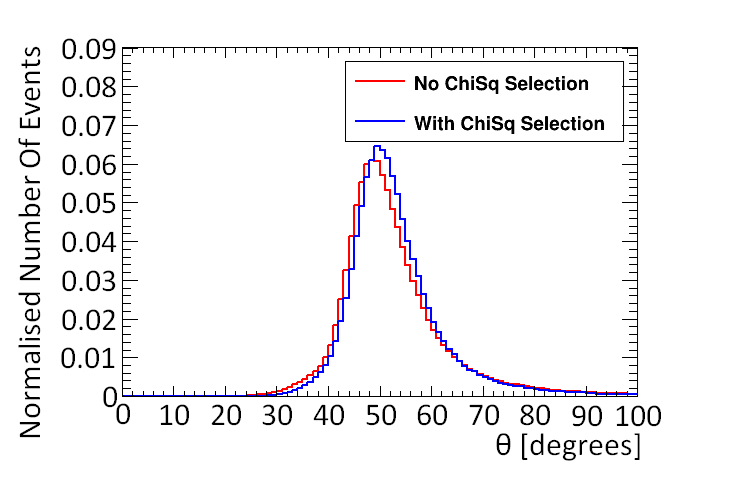
\includegraphics[width=0.5\linewidth]{Chapter6/Figs/Raster/simHemDeDxMedText.png}
  \captionof{figure}[dE/dx Of the simulated cosmic hemisphere both with and without a $\chi^2$/DOF selection criteria.]{dE/dx Of the simulated cosmic hemisphere both with and without a $\chi^2$/DOF selection criteria. Selection removes 90\,\% of events. The difference is minimal suggesting that a good series of selection criteria have been found regardless of $\chi^2$/DOF.}
  \label{fig:dedxGenVsRecoHem}
\end{figure}

% Before the data could be analysed a simulation of cosmic muons using a cosmic hemisphere was used in order to quantify segmentation and other detector effects. These effects can be quite significant as seen in figures \ref{subFig:phiGenVsRecoHem} and \ref{subFig:cirPhiGenVsRecoHem} the reconstruction of the RMon detector can be quite adversely affected by vertical events. If an event is vertical in one side of the detector then the other side will dominate as such it results in spikes at $\phi$ = 0$^\circ$, $\phi$ = 90$^\circ$, $\phi$ = 180$^\circ$, $\phi$ = 270$^\circ$. This bin migration is caused by the detector being a segmented cuboid. Any segmented cuboid detector will not cleanly represent a hemispherical distribution. Figures \ref{fig:cosmicBinMigrationSideA} and \ref{fig:cosmicBinMigrationSideB} show how the segmentation of the RMon/VIDARR detectors cause bin migration. For figure \ref{fig:cosmicBinMigrationSideA} angles of $\phi$ are solely determined by the direction in side A the same is true for side B in figure \ref{fig:cosmicBinMigrationSideB}. 
Any segmented cuboid detector will not cleanly represent a hemispherical distribution therefore to quantify how significant the distortion is, hemispherical source of cosmic muons was simulated, representing flat values in $\phi$ (0$^\circ$ -- 360$^\circ$) and $\theta$ (0$^\circ$ -- 90$^\circ$) as this represents all the angles the detector could encounter. A cuboid detector will have a different ``footprint'' in $\phi$ as $\theta$ increases towards the sky. When tracks are vertical ($\theta = 90^\circ$) the footprint is a 1.52\,m$^2$ in $\phi$ resulting in peaks at $\phi$ of 45$^\circ$, 135$^\circ$, 225$^\circ$, 315$^\circ$ and troughs $\phi$ of 0$^\circ$, 90$^\circ$, 180$^\circ$, 270$^\circ$. In figure \ref{fig:linCirPhiGenVsRecoHem} a clear oscillating pattern can be seen peaking at $\phi$ values of 45$^\circ$, 125$^\circ$, 275$^\circ$, 315$^\circ$ in the reconstruction which is not present in the generated distributions. This is a result of the cuboid shape of the detector. The small square footprint slowly morphs into a circle with an almost infinite radius when the events are horizontal ($\theta = 0^\circ$). As such any cuboid detector will distort $\phi$ distribution from square at $\theta = 90^\circ$ to circle at $\theta = 0^\circ$. The peaks at $\phi$ values of 0$^\circ$, 90$^\circ$, 180$^\circ$, 270$^\circ$ are not caused by the cuboid shape of the detector but rather by the segmentation. 
\begin{figure}[!h]
\centering
\begin{subfigure}{.5\textwidth}
  \centering
  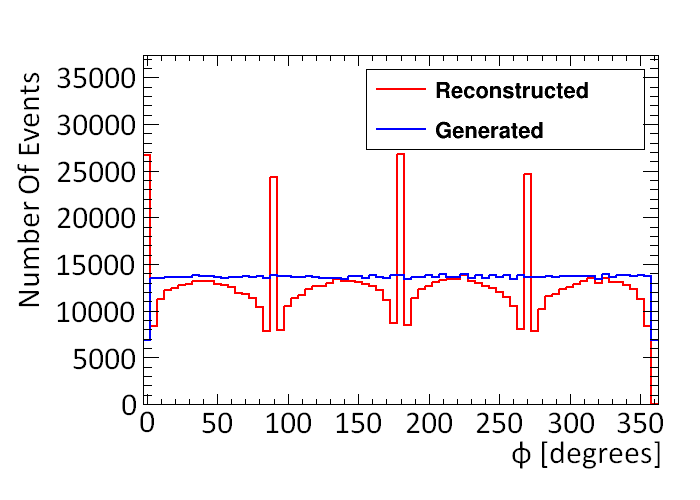
\includegraphics[width=\linewidth]{Chapter6/Figs/Raster/hemispherePhi_linHistMedText.png}
  \captionsetup{width=.9\linewidth}
  \caption{} 
  \label{subFig:phiGenVsRecoHem}
\end{subfigure}%
\begin{subfigure}{.5\textwidth}
  \centering
\includegraphics[width=\linewidth]{Chapter6/Figs/Raster/hemispherePhi_cirHistMedText.png}
  \captionsetup{width=.9\linewidth}
  \caption{}
  \label{subFig:cirPhiGenVsRecoHem}
\end{subfigure}
\caption[Generated $\phi$ vs reconstructed $\phi$ with the online track fitter.]{Generated $\phi$ vs reconstructed $\phi$ with the online track fitter for a cosmic hemisphere distribution. (a) shows the linear histogram for both (b) shows the circular histogram for reconstructed. The sharp peaks are caused by the segmentation and the undulating rate are caused by the detector shape.}
\label{fig:linCirPhiGenVsRecoHem}
\end{figure}

Segmentation causes accumulation at specific angles. If an event is vertical in one side of the detector than the other side will solely determine the $\phi$ component, it will dominate. Figure  \ref{fig:cosmicBinMigrationSideA} shows an example of what a side A dominating event looks like, whilst figure \ref{fig:cosmicBinMigrationSideB} shows a side B dominating event. This results in a migration of events at $\phi$ values of $0^\circ$, $90^\circ$, $180^\circ$, and $270^\circ$. This bin migration can be clearly seen in figures \ref{subFig:phiGenVsRecoHem} and \ref{subFig:cirPhiGenVsRecoHem} as the distribution spikes at the expected $\phi$ values. This segmentation effect is also compounded by the aforementioned cuboid shape of the detector. These bin migrations are not a significant concern provided they are properly understood, but it results in the data in $\phi$ being significantly distorted.  
 
\begin{figure}[!h]
 \centering
 \includegraphics[width=\linewidth]{Chapter6/Figs/Raster/phiSideABinMigrationMedText.png}
 \captionof{figure}[Side A bin migration due to the segmentation size of the detector.]{Side A bin migration due to the segmentation size of the detector. In this example side B has no $\phi$ component and so any value on side A determines $\phi$ exclusively thus warping the distribution.} 
 \label{fig:cosmicBinMigrationSideA}
\end{figure}

\begin{figure}[!h]
 \centering
 \includegraphics[width=\linewidth]{Chapter6/Figs/Raster/phiSideBBinMigrationMedText.png}
 \captionof{figure}[Side B Bin migration due to the segmentation size of the detector.]{Side B Bin migration due to the segmentation size of the detector. In this example side A has no $\phi$ component and so any value on side B determines $\phi$ exclusively thus warping the distribution.} 
 \label{fig:cosmicBinMigrationSideB}
\end{figure}

However, bin migration is significantly less pronounced in $\theta$. As shown by figure \ref{fig:thetaGenVsRecoHem} significant bin migration is only seen in binned $\theta$ values of 0$^\circ$, 5$^\circ$, 80$^\circ$, 85$^\circ$, 90$^\circ$ but bins 10$^\circ$ -- 75$^\circ$ are accurately reconstructed. The large discrepancy in bin migration between $\phi$ and $\theta$ is partially due to the size of the segments in the detector. The segments are 4\,cm wide by 1\,cm tall so they are able to more accurately reconstruct information vertically than in any other direction. Which is useful for reconstructing vertical information such as the height of buildings. But $\theta$ is also not distorted by the charging ``footprint'' of the cuboid detector, that distortion is exclusive to $\phi$. Though as will be outlined in section \ref{sec:cosmicTrackerUncertainties} the segmentation and effect of corner clipping events makes reconstruction of $\theta$ more difficult than expected. When comparing the generated hits for a cosmic hemisphere (figures \ref{subFig:rawHemisphereFiducialBarsSideA} and \ref{subFig:rawHemisphereFiducialBarsSideB}) to the reconstructed hits (figures \ref{subFig:hemisphereFiducialBarsSideA} and \ref{subFig:hemisphereFiducialBarsSideB}) they appear to match closely. Therefore, it is reasonable to assume that the tracker does not introduce any biases into the generated data set.

\begin{figure}[!h]
 \centering
 \includegraphics[width=0.5\linewidth]{Chapter6/Figs/Raster/hemisphereThetaCompareMedText.png}
 \captionof{figure}[Generated $\theta$ vs reconstructed $\theta$ for a cosmic hemisphere distribution.]{Generated $\theta$ vs reconstructed $\theta$ for a cosmic hemisphere distribution, biasing is minimal except at 0$^\circ$, 5$^\circ$, 80$^\circ$, 85$^\circ$ and 90$^\circ$ bins.} 
 \label{fig:thetaGenVsRecoHem}
\end{figure}

\begin{figure}[!h]
\centering
\begin{subfigure}{.5\textwidth}
  \centering
  \includegraphics[width=\linewidth]{Chapter6/Figs/Raster/rawHemisphereFiducialBarsSideAMedText.png}
  \captionsetup{width=.9\linewidth}
  \caption{}
  \label{subFig:rawHemisphereFiducialBarsSideA}
\end{subfigure}%
\begin{subfigure}{.5\textwidth}
  \centering
\includegraphics[width=\linewidth]{Chapter6/Figs/Raster/rawHemisphereFiducialBarsSideBMedText.png}
  \captionsetup{width=.9\linewidth}
  \caption{}
  \label{subFig:rawHemisphereFiducialBarsSideB}
\end{subfigure}
\begin{subfigure}{.5\textwidth}
  \centering
  \includegraphics[width=\linewidth]{Chapter6/Figs/Raster/hemisphereFiducialBarsSideAMedText.png}
  \captionsetup{width=.9\linewidth}
  \caption{}
  \label{subFig:hemisphereFiducialBarsSideA}
\end{subfigure}%
\begin{subfigure}{.5\textwidth}
  \centering
\includegraphics[width=\linewidth]{Chapter6/Figs/Raster/hemisphereFiducialBarsSideBMedText.png}
  \captionsetup{width=.9\linewidth}
  \caption{}
  \label{subFig:hemisphereFiducialBarsSideB}
\end{subfigure}
\caption[Hemisphere bars hit when using the generated $\phi$ and $\theta$ from CRY figure.]{Hemisphere bars hit when using the generated $\phi$ seen in figure \ref{subFig:phiGenVsRecoHem} and generated $\theta$ seen in figure \ref{fig:thetaGenVsRecoHem}. (a) and (b) show the generated bar hits for side A in (a) and side B in (b). The reconstructed tracker hits are shown in (c) and (d) with side A in (c) and side B in (d). The tracker is not disrupted by the dead channels and accurately reconstructs the hits with minimal detector corner clipping events removed. Dead and uninstrumented channels are simulated to improve accuracy and the simulation bounds match the fiducial bounds.}
\label{fig:HemisphereFiducialBarsSideAB}
\end{figure}

%The cosmic hemisphere distribution was chosen as it covers all possible angles in the ($\phi$,$\theta$) space that the detector will encounter. When reconstructing the ($\phi$,$\theta$) distribution of the cosmic hemisphere (figure \ref{fig:simulatedHemisphereDist}) a clear bin migration is visible. The reconstruction artefacts are shown in figures \ref{subFig:phiGenVsRecoHem} and \ref{fig:thetaGenVsRecoHem} can be seen to have a dependence on one another in figure \ref{fig:simulatedHemisphereDist}. Apart from the uncertainties introduced from the segmentation and shape of the detector no other uncertainties are significantly visible in figure \ref{fig:simulatedHemisphereDist}. However, this does not mean that other uncertainties are not present just that the most noticeable uncertainty is due to the segmentation and shape of the detector. 
As the bias added by tracker appears to be minimal the reconstructed ($\phi$,$\theta$) distribution in figure \ref{fig:simulatedHemisphereDist} mostly shows the compounding effects leading to bin migration. What is interesting about the distribution in figure \ref{fig:simulatedHemisphereDist} is how both the ``footprint'' and segmentation effects become minimal when $7.5^\circ \leq \theta \leq 37.5^\circ$. This is because the probability of vertical events in either side becomes very small once $\theta$ is steep which negates the segmentation effect. At $\theta \leq 7.5^\circ$ the segmentation causes issues as events start to travel down a single bar in one of the sides. The ``footprint''  effect is also negated at this point because every cosmic muon event footprint between $0^\circ \leq \theta \leq 90^\circ$ is technically a confluence between a square and circle as the horizon extends much further than the 1.52\,m$^2$ square of the detector's base. As a result, at $\theta \leq 37.5^\circ$  the horizon is the dominate distribution and the $\phi$ distortion caused by the square footprint of the detector is minimal. Therefore, there is an optimal range for reconstruction in figure \ref{fig:simulatedHemisphereDist} between $7.5^\circ \leq \theta \leq 37.5^\circ$ where the distribution is as uniform as possible. The lack of distortion in this area indicates the robustness of the tracking procedure. 

\begin{figure}[!h]
  \centering
  \includegraphics[width=0.7\linewidth]{Chapter6/Figs/Raster/pvsTFiduicalHemisphereMedText.png}
  \captionof{figure}[Tracker reconstructed ($\phi$,$\theta$) when simulating a cosmic hemisphere.]{Tracker reconstructed ($\phi$,$\theta$) when simulating a cosmic hemisphere which has a flat distribution in $\theta$ from 0$^\circ$ to 90$^\circ$ and a flat distribution in $\phi$ from 0$^\circ$ to 360$^\circ$.}
  \label{fig:simulatedHemisphereDist}
  %\vspace{0.478cm} %1 line = 0.478cm % 2 lines = 0.956cm % 3 lines= 1.434cm % 4 lines = 1.912cm % 5 lines = 2.39cm
\end{figure}

% \begin{figure}[!h]
%  \centering
%  \includegraphics[width=0.8\linewidth]{Chapter5/Figs/Raster/simulatedNormalDistirbution.png}
%  \captionof{figure}{\hl{theta has been reversed now!!!} Simulated distribution with an ideally generated cosmic distribution.} 
%  \label{fig:simulatedNormalDist}
% \end{figure}
